\documentclass[a4paper]{article}

\pdfminorversion=4

\usepackage[T1]{fontenc}
\usepackage[utf8]{inputenc}

\usepackage[scaled=.8]{beramono}

\usepackage{graphicx}
\usepackage{mathptmx}
\usepackage{fancyhdr}
\usepackage[top=5cm, bottom=3cm, left=2.5cm, right=2.5cm]{geometry}
\usepackage[usenames,dvipsnames,svgnames,table]{xcolor}
\usepackage{sectsty}
\usepackage{tocloft}

% Extra packages required for D5.2
\usepackage{amsmath}
\usepackage{xcolor}     % for colour
\usepackage{mdframed}   % for framing
\usepackage{algorithm}
\usepackage[noend]{algpseudocode}
\usepackage{url}
\usepackage{amssymb}
\usepackage{listings}
\usepackage{sty/lstsemantic}
\usepackage{amsthm}
\usepackage[table]{xcolor}

\usepackage[textsize=footnotesize]{todonotes}
% \usepackage[disable,textsize=footnotesize]{todonotes}

\usepackage[backend=bibtex,hyperref=auto,
% LNCS-style setup:
firstinits=true,style=numeric,
urldate=iso8601,isbn=false,doi=false]{biblatex}
\iffalse
% RefTeX for Emacs does not yet support multiple \addbibresource statements
\bibliography{aksw,kwarc,literature}
\fi
\addbibresource{aksw}
\addbibresource{kwarc}
\addbibresource{literature}
% poor man's LNCS styling
\setlength{\biblabelsep}{\labelsep}
\DeclareNameAlias{author}{last-first}
\DeclareNameAlias{editor}{last-first}
\DeclareNameAlias{translator}{last-first}
\DeclareFieldFormat{labelnumberwidth}{#1.}
\DeclareFieldFormat{title}{#1}
\DeclareFieldFormat
  [article,inbook,incollection,inproceedings,patent,thesis,unpublished]
  {title}{#1}
\DeclareFieldFormat{journaltitle}{#1}
\newbibmacro*{volume+number+eid}{%
  \printfield{volume}%
  \iffieldundef{number}
    {}
    {(%
      \printfield{number}%
     )%
    }%
  \setunit{\addcomma\space}%
  \printfield{eid}}
\DeclareFieldFormat{url}{\url{#1}}
\renewcommand{\finalnamedelim}{\addcomma\space}

% Style settings for D5.2
\global
\mdfdefinestyle{metricdefinition}{% 
linecolor=black, middlelinewidth=3pt,% 
leftmargin=1cm, rightmargin=1cm,
skipabove=6pt, skipbelow=6pt,
backgroundcolor=gray!30
}

\lstset{
  captionpos=b, 
  extendedchars=true,
  % basicstyle=\footnotesize \sffamily, 
  basicstyle={\scriptsize\ttfamily},
  % stringstyle=\bfseries,
  showstringspaces=false,
  breaklines=true,
  tabsize=2, % sets default tabsize
  frame=single % adds a frame around the code
}

\sloppy % ensures that no math words go in the margin

%%% settings for JSON listing
\colorlet{punct}{red!60!black}
\definecolor{delim}{RGB}{20,105,176}
\colorlet{numb}{magenta!60!black}

\lstdefinelanguage{json}{
	basicstyle={\scriptsize\ttfamily},
    numbers=none,
    showstringspaces=false,
    breaklines=true,
    frame=single,
    literate=
     *{0}{{{\color{numb}0}}}{1}
      {1}{{{\color{numb}1}}}{1}
      {2}{{{\color{numb}2}}}{1}
      {3}{{{\color{numb}3}}}{1}
      {4}{{{\color{numb}4}}}{1}
      {5}{{{\color{numb}5}}}{1}
      {6}{{{\color{numb}6}}}{1}
      {7}{{{\color{numb}7}}}{1}
      {8}{{{\color{numb}8}}}{1}
      {9}{{{\color{numb}9}}}{1}
      {:}{{{\color{punct}{:}}}}{1}
      {,}{{{\color{punct}{,}}}}{1}
      {\{}{{{\color{delim}{\{}}}}{1}
      {\}}{{{\color{delim}{\}}}}}{1}
      {[}{{{\color{delim}{[}}}}{1}
      {]}{{{\color{delim}{]}}}}{1},
}


%%%%%%%%%%%%%%%%%%%%%%%%%%%%%%%%%%%%%%%%%%%%%%%%%
% Changing TOC/LOF/LOT presentation
%%%%%%%%%%%%%%%%%%%%%%%%%%%%%%%%%%%%%%%%%%%%%%%%%
\renewcommand{\cfttoctitlefont}{\large\bfseries\scshape}
\renewcommand{\cftloftitlefont}{\large\bfseries\scshape}
\renewcommand{\cftlottitlefont}{\large\bfseries\scshape}
\renewcommand{\cftsecfont}{\bfseries\scshape}
\renewcommand{\cftsubsecfont}{\scshape}
\renewcommand{\cftsubsubsecfont}{\scshape}
\renewcommand\contentsname{Table of Contents}
\renewcommand\listfigurename{Table of Figures}
\renewcommand\listtablename{List of Tables}
\renewcommand{\cftsecleader}{\cftdotfill{\cftdotsep}}


%%%%%%%%%%%%%%%%%%%%%%%%%%%%%%%%%%%%%%%%%%%%%%%%%
% Embedding logos to the page style
%%%%%%%%%%%%%%%%%%%%%%%%%%%%%%%%%%%%%%%%%%%%%%%%%
\pagestyle{fancyplain}
\lhead{
\includegraphics[width=.3\textwidth]{images/diachron-logo.png}}
\rhead{Grant Agreement No. 601043}
\cfoot{\thepage}
\renewcommand{\headrulewidth}{0pt}
\allsectionsfont{\sffamily}

\begin{document}

%%%%%%%%%%%%%%%%%%%%%%%%%%%%%%%%%%%%%%%%%%%%%%%%%
% Title page
%%%%%%%%%%%%%%%%%%%%%%%%%%%%%%%%%%%%%%%%%%%%%%%%%
\begin{titlepage}

\begin{center}
  \begin{tabular}{ccc}
    
\includegraphics[width=.15\textwidth]{images/eu-logo.png} &
    
\includegraphics[width=.6\textwidth]{images/diachron-logo.png} &
    
\includegraphics[width=.15\textwidth]{images/fp7-logo.png}
  \end{tabular}
\end{center}

\vspace{4ex}
EU Project No:601043 (Integrated Project (IP))

\vspace{2ex}
DIACHRON

\vspace{2ex}
Managing the Evolution and Preservation of the Data Web DIACHRON

\begin{center}
  \begin{tabular}{@{}|ll|}
    \hline
    Dissemination level:  & Public\\
    Type of Document:  & Report \\
    Contractual date of delivery: & M16\\
    Actual Date of Delivery:  & \\
    Deliverable Number: & D5.2\\
    Deliverable Name: & Software prototype of the crawling, ranking and appraisal services\\
    Deliverable Leader: & UBONN\\
    Work package(s): & WP5\\ 
    Status \& version: & 0.1 (DRAFT)\\
    Number of pages: & \\
    WP contributing to the deliverable: & WP5 \\  
    WP / Task responsible: & T5.2, T5.3\\ 
    Coordinator (name / contact): & Jeremy Debattista / jeremy.debattista@iais-extern.fraunhofer.de (UBONN) \\  
    Other Contributors: & \parbox[c]{10cm}{\raggedright Christoph Lange, Natalja Friesen, and Santiago Londo\~no (UBONN), Ioannis Chrysakis, Kostas Stefanidis, and Giorgos Flouris (FORTH)}\\
    EC Project Officer: & Federico Milani \\
    \multicolumn{2}{|p{15cm}|}{\cellcolor{gray!20}
      \textbf{Keywords: data quality framework, quality metadata, quality metrics, dataset ranking, dataset crawling} 
    } \\
    \multicolumn{2}{|p{15cm}|}{\cellcolor{gray!50}
      \textbf{Abstract:} \newline
      The report describes the Data Quality Framework required to analyse and assess datasets for quality which would enable crawling and ranking.
    } \\
    \hline
  \end{tabular}
\end{center}

\end{titlepage}

%%%%%%%%%%%%%%%%%%%%%%%%%%%%%%%%%%%%%%%%%%%%%%%%%
% Version history
%%%%%%%%%%%%%%%%%%%%%%%%%%%%%%%%%%%%%%%%%%%%%%%%%
\begin{center}
  \begin{tabular}{|c|c|p{6cm}|p{7cm}|}
    \hline
    \multicolumn{4}{|c|}{\cellcolor{CornflowerBlue}Document History} \\
    \hline
    \rowcolor{LightSteelBlue}
    Ver. & Date & Contributor(s) & Description \\
    \hline
    0.1 & 24.06.2014 & Jeremy Debattista & Created TOC and LaTeX Setup \\
    \hline
    & & & \\
    \hline
    & & & \\ 
    \hline
  \end{tabular}
\end{center}

\newpage

%%%%%%%%%%%%%%%%%%%%%%%%%%%%%%%%%%%%%%%%%%%%%%%%%
% TOC
%%%%%%%%%%%%%%%%%%%%%%%%%%%%%%%%%%%%%%%%%%%%%%%%%
\tableofcontents

\newpage

%%%%%%%%%%%%%%%%%%%%%%%%%%%%%%%%%%%%%%%%%%%%%%%%%
% LOF and LOT contiguously
%%%%%%%%%%%%%%%%%%%%%%%%%%%%%%%%%%%%%%%%%%%%%%%%%
\listoffigures
\listoftables

\newpage

%%%%%%%%%%%%%%%%%%%%%%%%%%%%%%%%%%%%%%%%%%%%%%%%%
% Main Sections
%%%%%%%%%%%%%%%%%%%%%%%%%%%%%%%%%%%%%%%%%%%%%%%%%
%!TEX root = ../../diachron-D5_2.tex

\section{Introduction}
\label{sec:Introduction} 

%!TEX root = ../../diachron-D5_2.tex

\subsection{Scope and Objectives}
\label{sec:ScopeAndObjectives} 

This document describes the Diachron quality assessment service and its general applications.
Taking a broad view of quality as ``fitness for use''~\cite{Juran1974:biblatex}, we have designed a generic, extensible quality assessment framework, which is intended to serve all purposes envisaged in the Diachron project but also beyond.
We initially support quality assessment on RDF data, no matter whether they are streamed, e.g.\ from a big dataset dump, or obtained from a SPARQL endpoint.
We represent the output of quality assessment as an RDF graph of \emph{quality metadata}, which can be stored as annotations to the original dataset.
This approach enables flexible reuse of the quality metadata for visual quality analysis, quality-based filtering and ranking of datasets, and many other applications, without unnecessary recomputation.
This document also describes the implementation of a large number of concrete quality metrics within the framework.
We have so far implemented \todo{CL@JD: or even \emph{all}? - nope we have i say around 65\%}a substantial number of the quality metrics required for the Diachron pilot applications, focusing on those metrics that can be computed by analysing the dataset itself, the vocabularies it uses, and its immediate outgoing links to other datasets.
The dataset itself is analysed in a triple-by-triple streaming fashion, which ensures scalability over big datasets \todo{CL@JD: I thought I'd mention one limitation - agreed}at the expense of ruling out certain complex quality metrics.
\todo{CL: Hanzo to write something about quality-driven crawling}
%!TEX root = ../../diachron-D5_2.tex

\subsection{Context of this Document}
\label{sec:ContextDoc} 

\todo{CL: my first shot; improvised w/o looking into previous deliverables; need to verify against them}The overall architecture of Diachron, as outlined in Deliverable 6.1~\todo{CL: add to bibtex}\cite{diachron-d6.1}, comprises services that access and operate on diachronic data, as well as pilot applications that solve domain-specific problems and make use of the services to handle data specific to these problems.  An initial specification of the interfaces of these services – RESTful web services that speak JSON, to be exact – has also been provided in Deliverable 6.1.  Here, we describe the \emph{implementation} of the \emph{quality assessment service} and explain, in a generic, domain-independent way, how to use it to assess the quality of data.

% How does this work relate to WP5 in general and the whole project
% add the image of the whole diachron architecture (6.1)
% ? and highlight the part(s) covered by this deliverable

%%% Local Variables: 
%%% mode: latex
%%% TeX-master: "../../diachron-D5_2"
%%% End: 

%!TEX root = ../../diachron-D5_2.tex

\subsection{Document Structure}
\label{sec:DocumentStructure} 

Section~\ref{sec:DQF} defines a generic, extensible data quality framework, which is not specific to any Diachron application domain.  The framework allows for implementing arbitrary concrete quality metrics; any such metric is implemented partly in Java and partly as an extension of the data quality (daQ) core vocabulary.  The input dataset, currently assumed to be represented in RDF, is fed into all quality metric implementations of the user's choice; the output is represented as a set of RDF metadata in terms of daQ and its concrete, metric-specific extensions, so that it can be stored and reused flexibly.  This core quality assessment step is accessible through a web service interface.  Supported uses of a dataset's quality metadata include visual quality analysis (over multiple revisions of a dataset if desired) as well as \todo{CL@JD: Interestingly visual analysis is covered in section 2 as a part of the ``framework''; filtering and ranking is not.  Why this difference? - JD: you are right, i had to move the visualisation part to section 4 with the ui}filtering and ranking datasets by their quality.  

Section~\ref{sec:Libraries} lists the libraries that served as technical prerequisites for implementing the quality assessment service.

Section~\ref{sec:RankingService} describes in detail the general processes of data quality assessment and quality-based ranking, the design of a self-contained user interface giving access to the quality assessment service (optionally also the cleaning service described in Deliverables 3.1~\cite{d3.1} and 3.2~\todo{CL: add to bibtex}\cite{diachron-d3.2}, as well as all concrete metrics that we have implemented so far, with a special focus on those required for the Diachron pilot applications.

\todo{CL@Hanzo: also introduce section~\ref{sec:CrawlingService} once you have written it}

%%% Local Variables: 
%%% mode: latex
%%% TeX-master: "../../diachron-D5_2"
%%% End: 

%!TEX root = ../../diachron-D5_2.tex

\section{Data Quality Framework}
\label{sec:DQF} 

%!TEX root = ../../diachron-D5_2.tex

\subsection{High-Level Architecture}
\label{sec:HLA} 

The purpose of the Quality Framework is to provide an integrated platform that: 
\begin{enumerate}
\item assesses Linked Open Data (via RDF Dumps or SPARQL endpoints) in a scalable manner;
\item provides queryable quality metadata on the assessed datasets;
\item provides visualisations on the quality 
\end{enumerate}
Furthermore, we aim to create an infrastructure and a platform that (i) can be easily extensible by different third parties by creating their custom and more specific pluggable metrics required to assess their particular dataset domain, and (ii) having the the necessary ontology framework to represent the metadata about the quality of the assessed linked datasets.

Currently, there is no uniform infrastructure to address the quality assessment problem, allowing the extension or redefinition of custom-specific metrics such as those required by the DIACHRON use cases.
Tools such as Trellis~\cite{Gil2002}, WIQA~\cite{Bizer2008:PhDThesis:biblatex} and Sieve~\cite{Mendes2012} implement a number of metrics but lacks flexibility w.r.t.\ the level of automation, and user friendliness~\cite{Zaveri2012:LODQ} 

\begin{figure*}[tbph]
\center
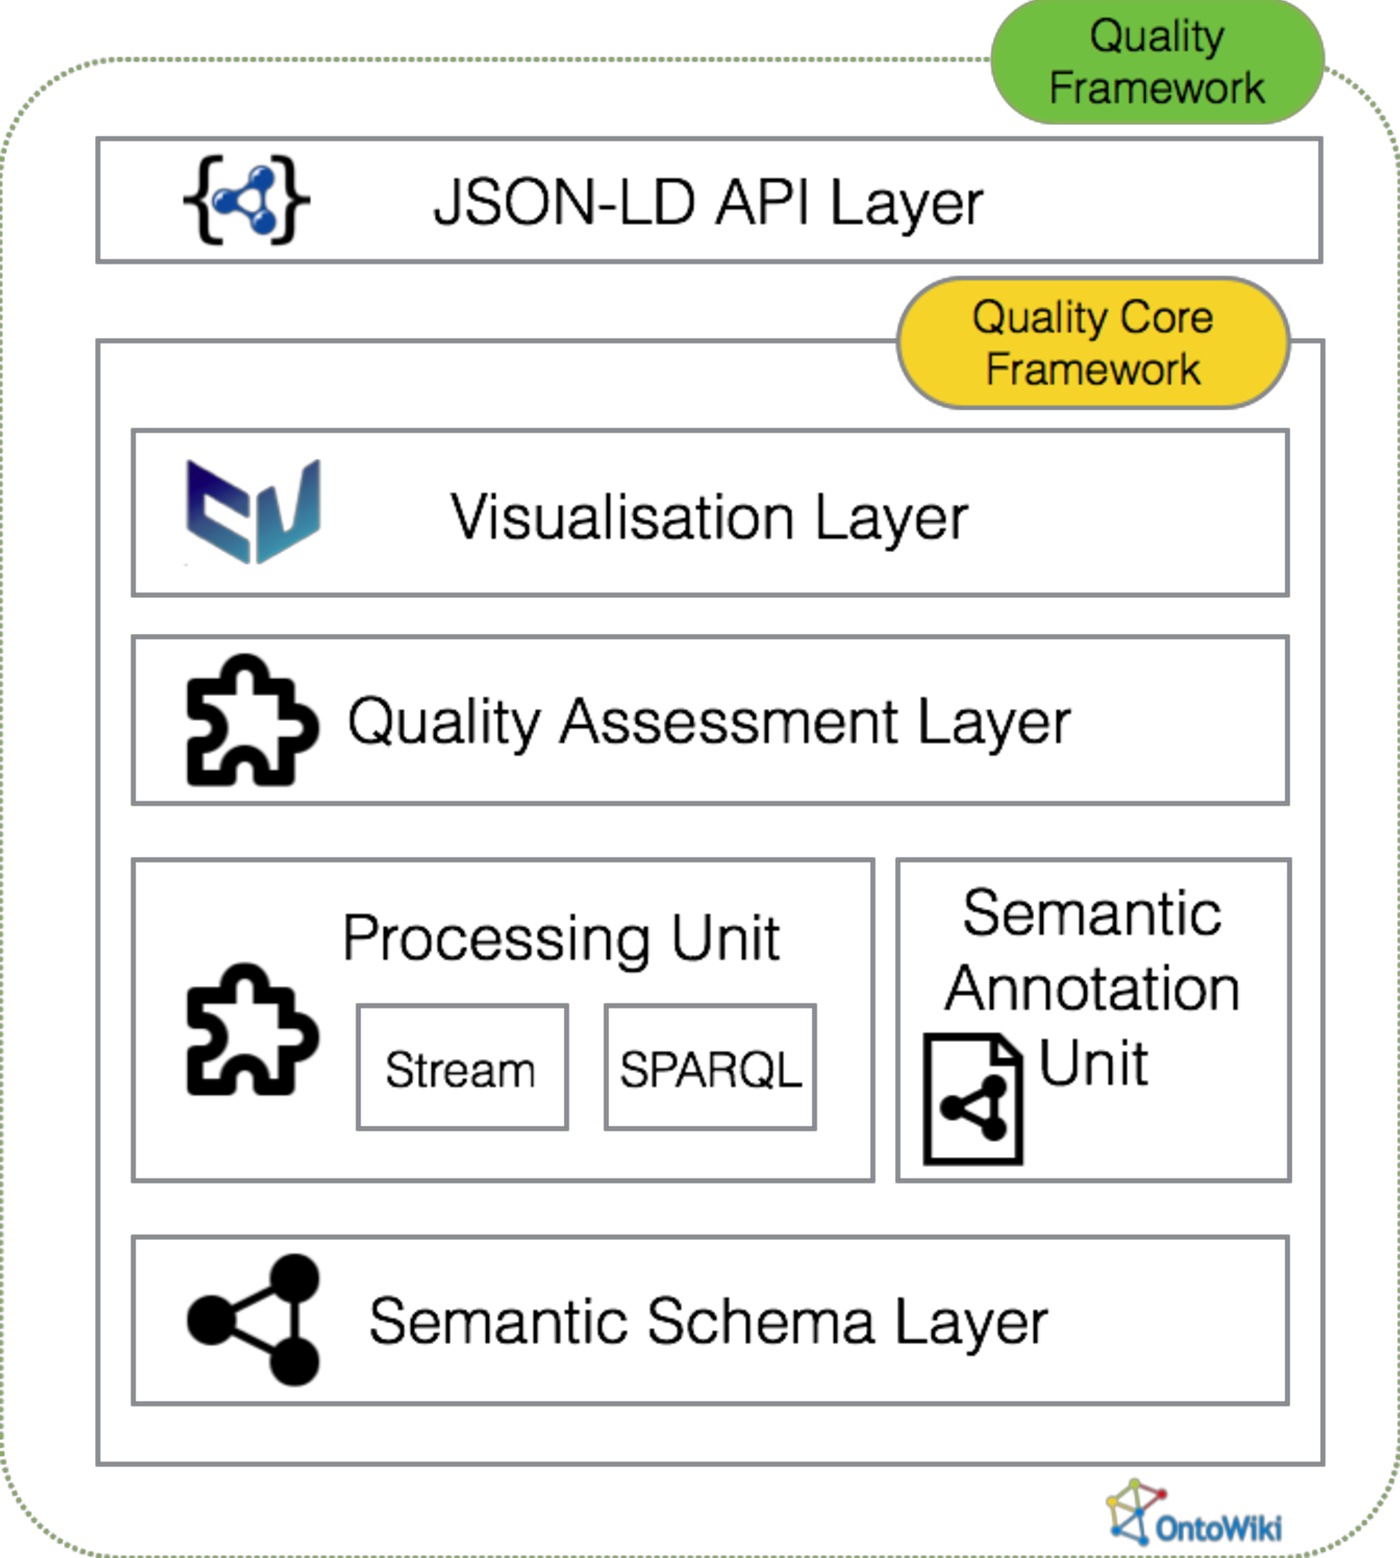
\includegraphics[scale=0.3]{images/qualityFrameworkHLA.pdf} 
\caption{Quality Framework High Level Architecture Design} 
\label{fig:qualityFramework}
\end{figure*}

Figure~\ref{fig:qualityFramework} illustrates the high level architecture of the Quality Framework.
The two main components are the API layer (cf. Section~\ref{sec:RestAPI}) and the Core framework.
The core framework is made up of four modules: \emph{Semantic Schema Layer}, \emph{Processing Unit}, \emph{Semantic Annotation Unit}, \emph{Quality Assessment Layer}, and an optional \emph{Visualisation Layer} which we will discuss in Section~\ref{sec:UI}.

\subsubsection{Semantic Schema Layer}
The Quality Framework is based on semantic technologies and thus has an underlying semantic vocabulary layer which currently is made up of two ontologies: (i) the Dataset Quality Ontology (daQ)\todo{CL@JD: in addition to these URLs, which currently only serve RDF/XML, please also mention the URLs of the TriG source.  BTW I had to create the purl's for dqm and qr today. - JD: i did not understand this comment}\footnote{\url{http://purl.org/eis/vocab/daq}}; and (ii) the Quality Problem Report Ontology (qr)\footnote{\url{http://purl.org/eis/vocab/qr}}. 
The former describes the quality metadata representation whilst the latter describes quality problems found in the dataset itself. 
The semantic schema layer is meant to be domain independent, where it could be reused in other similar frameworks. 
The daQ ontology (cf. Section~\ref{sec:DAQ}) is the core vocabulary of this schema layer, and any other ontology part of this layer builds upon it.

The daQ ontology is a comprehensive generic vocabulary framework, based on three abstract concepts (Category, Dimension and Metric). 
Any newly implemented specific metric should have its representation in RDF, extending the daQ ontology. In DIACHRON, all metrics are defined in the Diachron Quality Metric vocabulary (DQM)\footnote{\url{http://purl.org/eis/vocab/dqm}}. 
Such vocabularies are straightforward to integrate into the Quality Framework, since they adopt and extend the generic daQ vocabulary (by inheriting classes and properties) as the way quality metadata is represented (cf. Section~\ref{sec:extendingDAQ}).
The Quality Problem Report Ontology (qr) is made up of two classes a \texttt{qr:QualityReport} and \texttt{qr:QualityProblem}. 
The former represents a report on the problems detected during the assessment of quality on a dataset, whilst the latter represents the individual quality problems making up that report. 
Four properties are also defined in the ontology. 
The \texttt{qr:computedOn} represents the dataset URI on quality assessment has been made. 
This property is attached to a \texttt{qr:QualityReport}. \texttt{qr:hasProblem} links a \texttt{qr:QualityProblem} to a \texttt{qr:QualityReport}. 
The mentioned property identifies problem instances in a report. 
Each \texttt{qr:QualityProblem} \texttt{isDescribedBy} an instance of a \texttt{daq:Metric}\footnote{refer to Section~\ref{sec:DAQ}}. 
The property \texttt{qr:problematicThing} represent the actual problematic instance from the dataset. This could be a list of resources (\texttt{rdf:Seq}) or a list of reified statements.
Listing~\ref{lst:dataset_qr} represents an excerpt from a typical dataset showing the instance of \texttt{ex:JoeDoe} who is a \texttt{foaf:Researcher} working for \texttt{ex:UniBonn}.
In these two instances there are three problematic triples:
\begin{description}
\item [(A) $\langle$ \texttt{ex:JoeDoe a foaf:Researcher} $\rangle$] - The problem in this triple is caused by the usage of an undefined class, in this case \texttt{foaf:Researcher};
\item [(B) $\langle$ \texttt{ex:JoeDoe rdfs:label "JoeDoe"} $\rangle$] - The literal ("JoeDoe") in the triple causes the malformed capitalisation metric to point out a problem in this triple (as labels should be written in a human-friendly style);
\item [(C) $\langle$ \texttt{ex:UniBonn rdfs:label "UniBonn"} $\rangle$] - \todo{CL@JD: Is this third example necessary?  It's redundant with the second. - JD: you're right but i did it just for completeness sake - if it bothers you i'll remove it}The literal ("UniBonn") in the triple causes the malformed capitalisation metric to point out a problem in this triple.
\end{description}
Listing~\ref{lst:qualityreport} represent these three problems using the Quality Problem Report ontology.
\lstinputlisting[caption={An excerpt of a typical dataset},label=lst:dataset_qr, language=N3]{listings/qrtest.trig}
\lstinputlisting[caption={An corresponding Quality Report for Listing~\ref{lst:dataset_qr}},label=lst:qualityreport, language=N3]{listings/qualityreport.trig}

\subsubsection{Processing Unit}
\label{sec:processingUnit}
The Processing Unit is an integral part of the Quality Framework.
In this framework, we provide two main scalable processing units: a sequential stream processor (cf. Section~\ref{sec:StreamProcessor}) and a SPARQL processor\footnote{The SPARQL processor is still being investigated and will not be ready by the deliverable deadline.}.
The former streams triples from RDF data dumps one by one in a sequential fashion.
The latter allows the framework to assess quality on data that is available only in SPARQL endpoints. 
This unit is one of the two extensible modules (the other being Quality Assessment Layer) in the Quality Framework.
For DIACHRON, the plan is to extend the sequential stream processor, enabling the de-reification of RDF statements into RDF triples.

Typically, an initialised processor has 2 inputs: the dataset URI (for the sequential stream processor) or the dataset SPARQL endpoint (in the case of the SPARQL processor), and a metric configuration file selecting the metrics to be computed on the dataset.
Listing~\ref{lst:conf_metric} shows an example of a typical metric configuration file.
\lstinputlisting[caption={An typical metric configuration file},label=lst:conf_metric, language=N3]{listings/conf.trig} 
Each data processor in the Quality Framework has a defined 3-stage procedure (Listing~\ref{lst:int_ioprocessor}): (i) processor initialisation; (ii) processing; and (iii) memory clean up.
In the first process (processor initialisation), the processor create the necessary objects in memory to process data and load the required metrics that are instructed in the configuration file.
Once the initialisation is ready, the processing is done by passing the streamed triples into the metrics.
A final memory cleanup ensures that no unused objects are using unnecessary computational resources.
\lstinputlisting[caption={IO Processor Interface},label=lst:int_ioprocessor, language=Java]{listings/ioprocessor.java} 

\subsubsection{Quality Assessment Layer}
\label{sec:qaLayer}
The Quality Assessment Layer is undeniably the most important layer in this Quality Framework.
The framework can be extended by any third party providing their own custom specific metric.
This is already done in the DIACHRON project, where a number of metrics (cf. Section~\ref{sec:DQMetrics}) required to assess the various use cases specified in~\cite{diachron-d5.1} are implemented.
The Quality Assessment Layer provides two interfaces and an abstract class (cf. Figure~\ref{fig:classDiagram}) which facilitate the quality framework to be a pluggable and extensible platform.
The interface \texttt{QualityMetric} is the core interface class which describes the metric classes.
Each metric implementing this interface, must implement the following methods:
\begin{description}
\item[compute] assesses the quad\footnote{A quad is a triple with an added context value (eg. a named graph URI where the triple is found).}/triple which is passed by the stream processor by the defined metric;
\item[metricValue] returns the value computed by the quality metric;
\item[toDAQTriples] returns a list of daQ triples, containing quality metadata about the assessed metric, which \todo{CL@JD: really \emph{will}, or rather \emph{can}?  The QA framework is not itself in charge of storage.} will be used to create the quality metadata for the assessed dataset;
\item[getMetricURI] returns the URI of the Quality Metric from the ontology description (e.g. \url{http://purl.org/eis/vocab/dqm#DereferenceablityMetric});
\item[getQualityProblems] returns a typed list of either Resources or Quads, which will be used to create a quality report of the metric;
\end{description}

\begin{figure*}[tbph]
\center
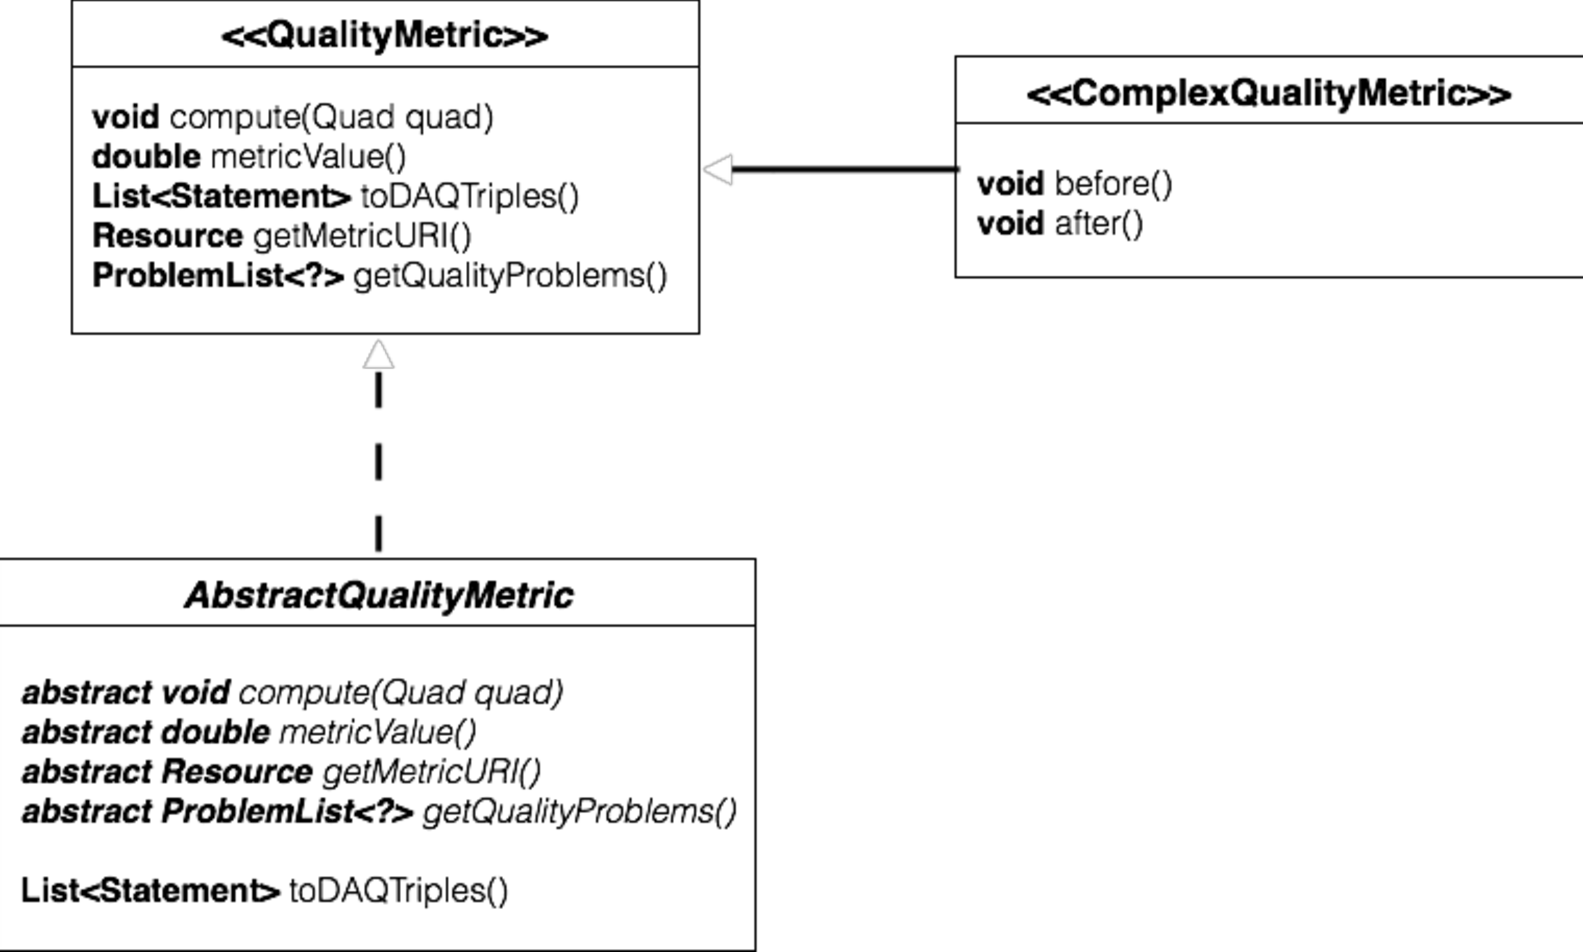
\includegraphics[scale=0.3]{images/classdiagram.pdf} 
\caption{Quality Assessment Layer Class Diagram – A Quality Framework as a Pluggable Platform} 
\label{fig:classDiagram}
\end{figure*}

Furthermore, computing a metric might require some pre-processing or post-processing.
Therefore, an interface (\texttt{ComplexQualityMetric}) extending \texttt{QualityMetric} was developed.
This interface allow metric developers to perform such processing using the \texttt{\textbf{void} before(Object ... args)} and \texttt{\textbf{void} after(Object ... args)} methods.

In order to facilitate further such development of pluggable metrics, the \texttt{AbstractQualityMetric} class was developed, implementing the \texttt{QualityMetric} interface.
In this abstract class, the method \texttt{List$\langle$Statement$\rangle$ toDAQTriples()} is implemented, generating quality metadata \todo{CL@JD: not sure this term will be understood.  Maybe speak of ``quality metadata'' here, and only introduce it (but then with an explanation) below for data cubes. - JD: agreed}observation instances (cf. Section~\ref{sec:DAQ}) for the metric being assessed.
Having this generic implementation of the method would ensure that the quality metadata is described correctly with respect to its definition in the Dataset Quality Ontology.

\subsubsection{Semantic Annotation Unit}
The Semantic Annotation Unit takes the generated triples (from the \texttt{toDAQTriples()} method) in order \todo{CL@JD: again I wouldn't give the impression that we are taking care of storage.  These metadata \emph{can} be stored inside the dataset, but we are not in charge of it. - JD: better?}to create the quality metadata for an assessed dataset.
This unit will handle the necessary communications with the datastore to insert the generated quality metadata in the dataset itself.
The unit provides a number of helper classes that provide inferencing queries on vocabularies that describe metrics (in the case of DIACHRON, the DQM vocabulary) based on the core ontology - Dataset Quality Ontology (daQ).
Therefore, RDF descriptions of metrics extending the daQ (cf. Section~\ref{sec:extendingDAQ}) ontology are absolutely required.
These inferencing queries enable the framework to create a complete metadata description (cf. Section~\ref{sec:DAQ}) of an assessed quality metric.

% in this section we need to describe the general architecture (stream processor, daq, cache, metrics, plugins etc...) of the quality framework - including how this framework will connect to other modules in diachron

%%% Local Variables: 
%%% mode: latex
%%% TeX-master: "../../diachron-D5_2"
%%% End: 



%!TEX root = ../../diachron-D5_2.tex

\subsection{Sequential Stream Processor}
\label{sec:StreamProcessor} 
In order to accurately assess linked dataset for quality measures, the assessment should on all triples in the assessed datasets.
One must keep in mind that the computation of metrics on large datasets might be computationally expensive; thus, such stream processors computing dataset's quality must be scalable.
In Figure~\ref{fig:closerLook}, a closer look towards the quality assessment process is illustrated.
A user first chooses a dataset and the metrics which are required for the assessment of quality.
The submitted information is passed to the Quality Framework via its API and initialise the processing unit (stream processor) in the core framework.
The stream processor is then initialised by: (1) creating the necessary objects in memory, and (2) initialise the chosen metrics. 
In Figure~\ref{fig:closerLook}, ``Metric 1'' is shadowed out – to illustrate that it was not chosen by the user for this particular use case.
Once the objects created, the stream processor fetches the dataset and in a sequential fashion it starts streaming quads one by one to all initialised metrics in parallel.
After all statements are assessed, the semantic annotation unit requests the metric value for each metric and creates (or updates – in case the dataset already has one) the Quality Graph.
This named graph represents the quality metadata of a dataset using the representation defined in Section~\ref{sec:DAQ}, and it is stored in the dataset itself.
Having this metadata, it will allow us to rank and crawl datasets based on different quality attributes.

\begin{figure*}[tbph]
\center
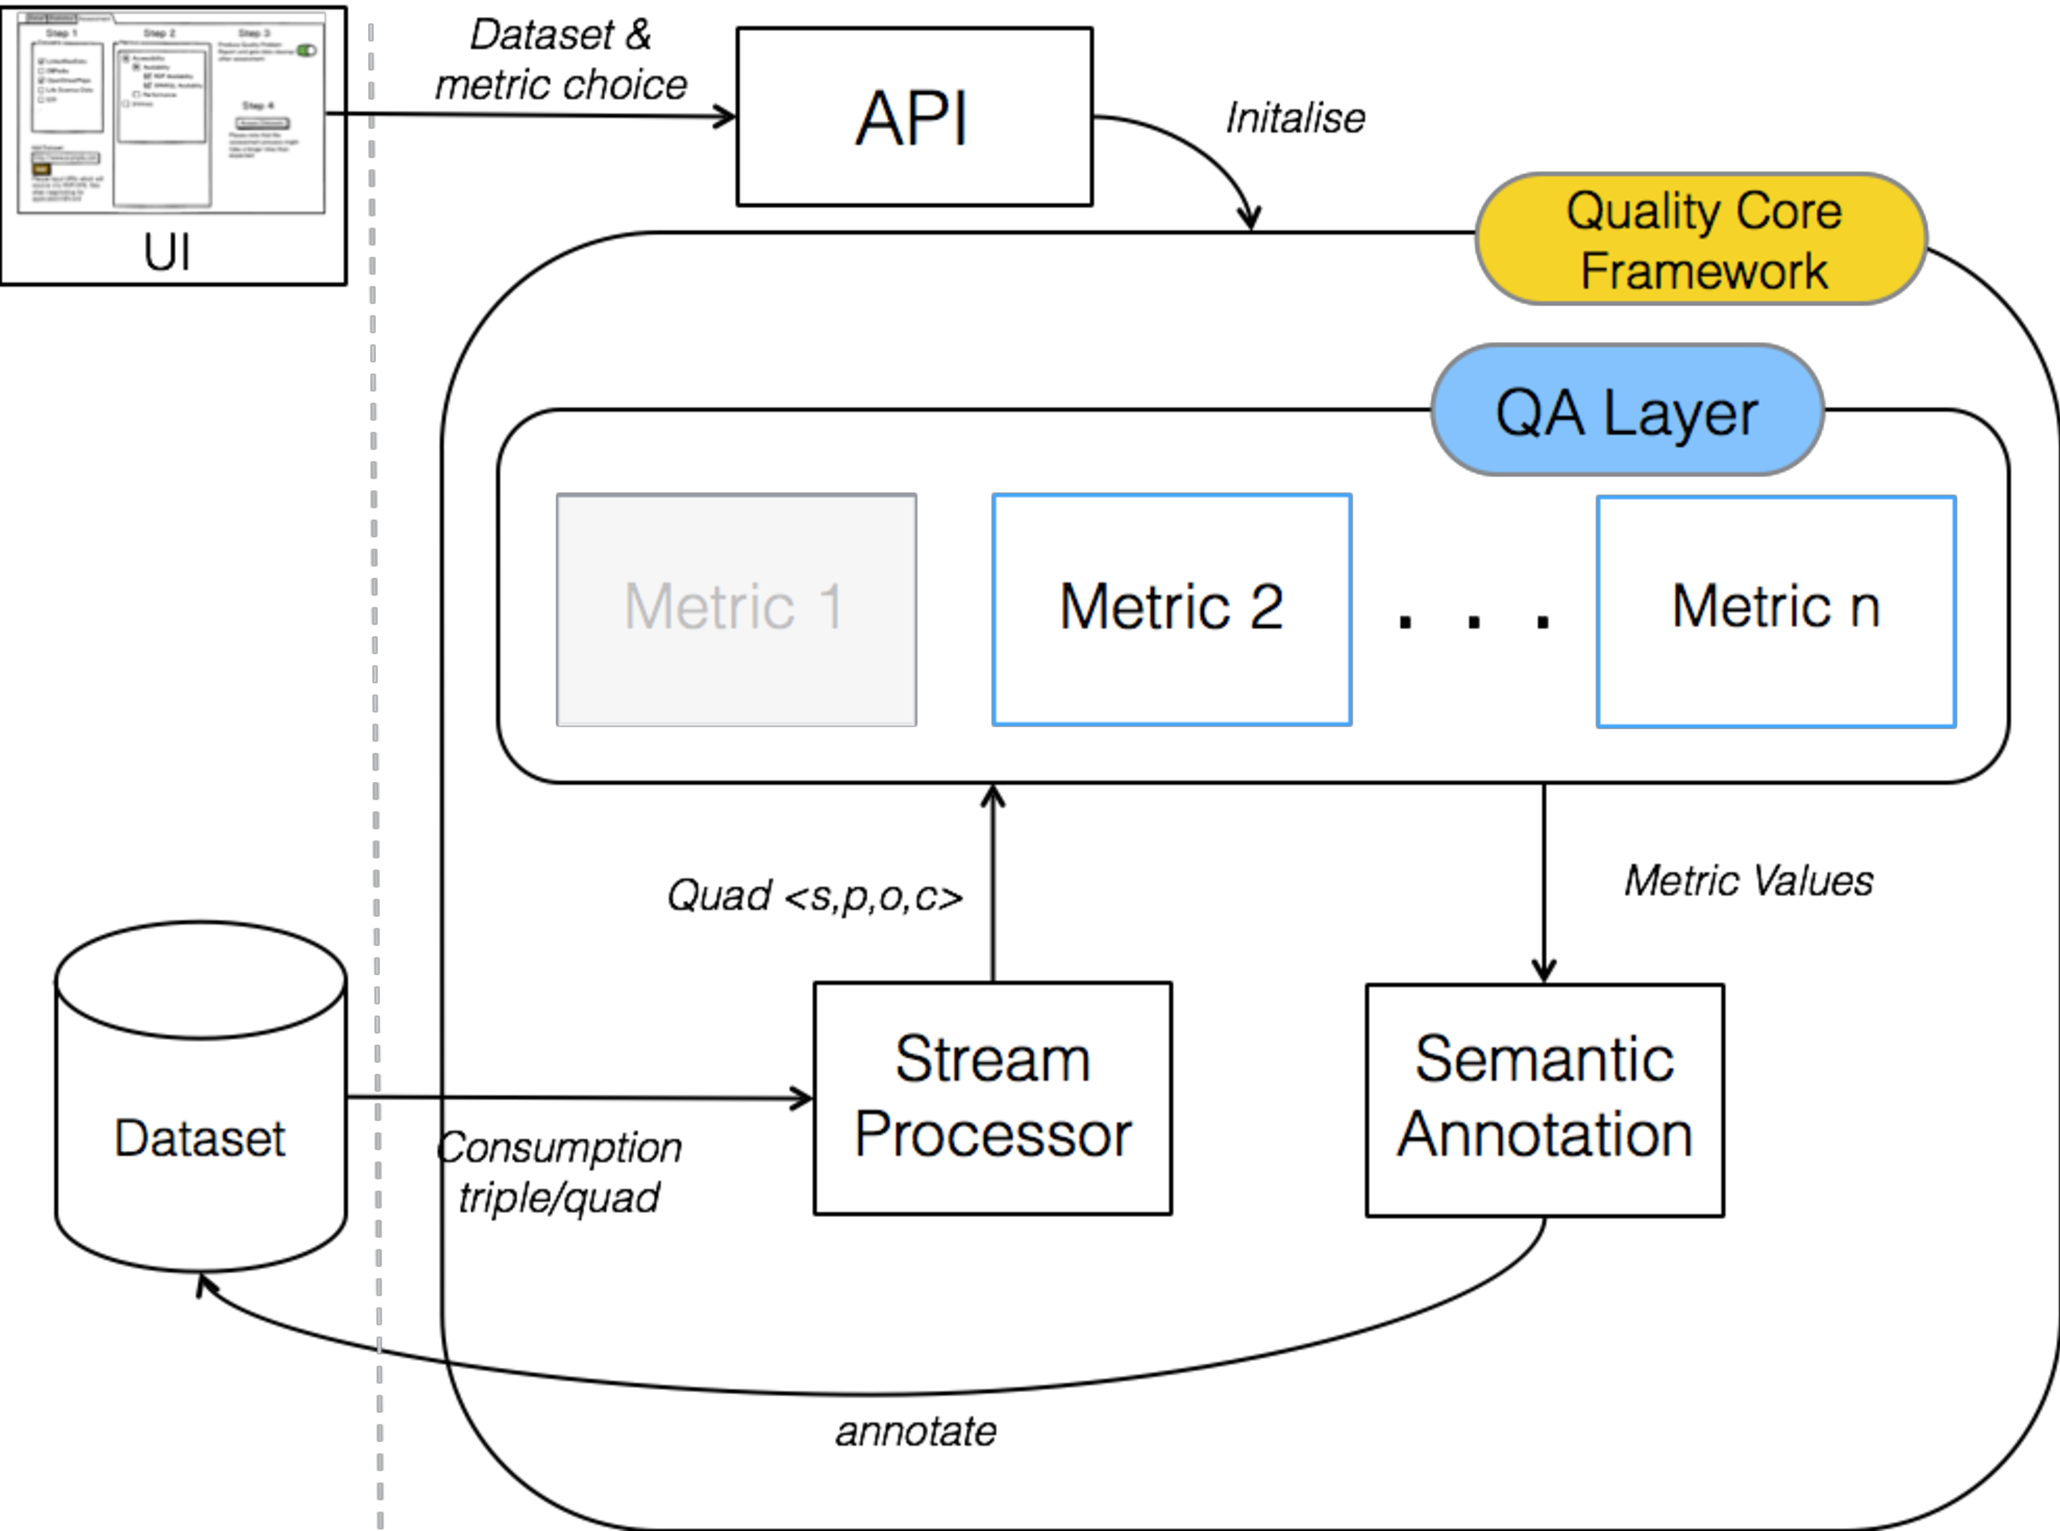
\includegraphics[scale=0.3]{images/closerLook.pdf} 
\caption{Closer look at the Quality Assessment process} 
\label{fig:closerLook}
\end{figure*}

Apache Jena\footnote{\url{http://jena.apache.org}} (cf. Section~\ref{sec:Jena}) provides a dedicated module for reading and writing RDF Data (RDF I/O Technology – RIOT\footnote{\url{http://jena.apache.org/documentation/io/rdf-input.html}}).
The RIOT API functionality provides a number of classes.
Typically the \texttt{RDFDataMgr} is used, which contains the main set of functions to read and load models and datasets.
For the sequential stream processor, the Jena RIOT API was used.

\subsubsection{The Initialisation Process – \texttt{setUpProcess()}}
The first operation on the initialisation is the execution of the \emph{setUpProcess()} method.
Listing~\ref{lst:setUp} is the pseudocode of the the process.
The sequential stream processor starts its initialisation by first trying to identify the serialisation used by the available RDF data dump.
The method \texttt{guessRDFSerialisation} analyses the file serialisation by mapping the file name to one of the RDF serialisations for which Jena has built-in support (e.g. RDF/XML, NTriples, Turtle, NQuads, etc\dots)
According to the file's serialisation, the process then assigns different types of \texttt{PipedRDFIterator}\footnote{\url{https://jena.apache.org/documentation/javadoc/arq/org/apache/jena/riot/lang/PipedRDFIterator.html}} and either a\texttt{PipedQuadsStream}\footnote{\url{https://jena.apache.org/documentation/javadoc/arq/org/apache/jena/riot/lang/PipedQuadsStream.html}} or \texttt{PipedTriplesStream}\footnote{\url{https://jena.apache.org/documentation/javadoc/arq/org/apache/jena/riot/lang/PipedTriplesStream.html}} 
These two objects are required for the scalable execution of the sequential stream processor as together they act as a the ``producer''\footnote{As in the producer in the ``Producer-Consumer problem'' \url{http://en.wikipedia.org/wiki/Producer?consumer_problem}. The consumer is on a separate thread, feeding the metrics.} of sequential RDF triples from the RDF data dump.
Once these are initialised, a flag is set to true to signal that the processor unit is in progress.
Finally, the chosen metrics are loaded into memory.
The loading of metrics is done dynamically during runtime, using the Java specific \texttt{newInstance()}\footnote{\url{http://docs.oracle.com/javase/8/docs/api/java/lang/Class.html#newInstance--}} method. 

\begin{algorithm}
\caption{The Initialisation of the Sequential Stream Process}
\label{lst:setUp}
\begin{algorithmic}[1]
\Procedure{setUpProcess}{}
\State rdfSerialisation = guessRDFSerialisation(datasetURI) ;

\If {rdfSerialisation is Quads} 
\State iterator = new PipedRDFIterator$\langle$Quad$\rangle$() ;
\State rdfStream = new PipedQuadsStream((PipedRDFIterator$\langle$Quad$\rangle$) iterator) ;
\EndIf
\If {rdfSerialisation is Triple} 
\State iterator = new PipedRDFIterator$\langle$Triple$\rangle$() ;
\State rdfStream = new PipedTriplesStream((PipedRDFIterator$\langle$Triple$\rangle$) iterator) ;
\EndIf

\State set initialised boolean to true ;

\State loadMetrics() ;
\EndProcedure
\end{algorithmic}
\end{algorithm}

\subsubsection{The Processing of Triples – \texttt{startProcessing()}}
After the initialisation process, the method \texttt{startProcessing()} is invoked.
The RDFStream \texttt{rdfStream} object starts parsing the RDF dump and producing triple or quad statements in the \texttt{iterator}.
On a different thread, the ``consumer'' – the sequential stream processor – consumes these statements from the \texttt{iterator}, converts them into quads of $\langle s,p,o,c \rangle$, and passes them to all initialised metrics.
The consumption process is repeated until all statements are exhausted from the \texttt{iterator}.
The semantic annotation unit is then signalled to start its annotation.
Listing~\ref{lst:processing} describes this process in pseudocode.

\begin{algorithm}
\caption{Processing Triple/Quad Statements}
\label{lst:processing}
\begin{algorithmic}[1]
\Procedure{startProcessing}{}
\If {initialised == false} \State{throw exception} ; \EndIf

\State create new producer thread for rdfStream ;

\While{(iterator has another statement)} 
\State{quad = Object2Quad(iterator.next()) ;}
\State{pass quad to all metrics and compute metric ;} 
\EndWhile

\State invoke semantic annotation unit ;
\EndProcedure
\end{algorithmic}
\end{algorithm}

\subsubsection{Clean Up – \texttt{cleanUp()}}
The final process is to clean up the objects from memory.
The processor follows a simple approach by assigning \texttt{null} to all objects and shutting down all running threads.

% describe how the stream processor work and the idea behind the processor. 
%!TEX root = ../../diachron-D5_2.tex

\subsection{The Dataset Quality Ontology}
\label{sec:DAQ} 
% describe the ontology which is used to describe the quality metadata of a dataset
The idea behind the Dataset Quality Ontology~\cite{DebattistaEtAl:daQ:LDOW:2014}\footnote{\url{http://purl.org/eis/vocab/daq}} (daQ) is to provide a comprehensive generic vocabulary framework, allowing a uniform definition of specific data quality metrics and thus suggest how quality metadata should be represented in datasets.
This metric definition would then allow publishers to attach data quality metadata with quality benchmarking results to their linked dataset.
Figure~\ref{fig:daqExtended} depicts the current state of the daQ vocabulary.

\begin{figure*}[tbph]
\center
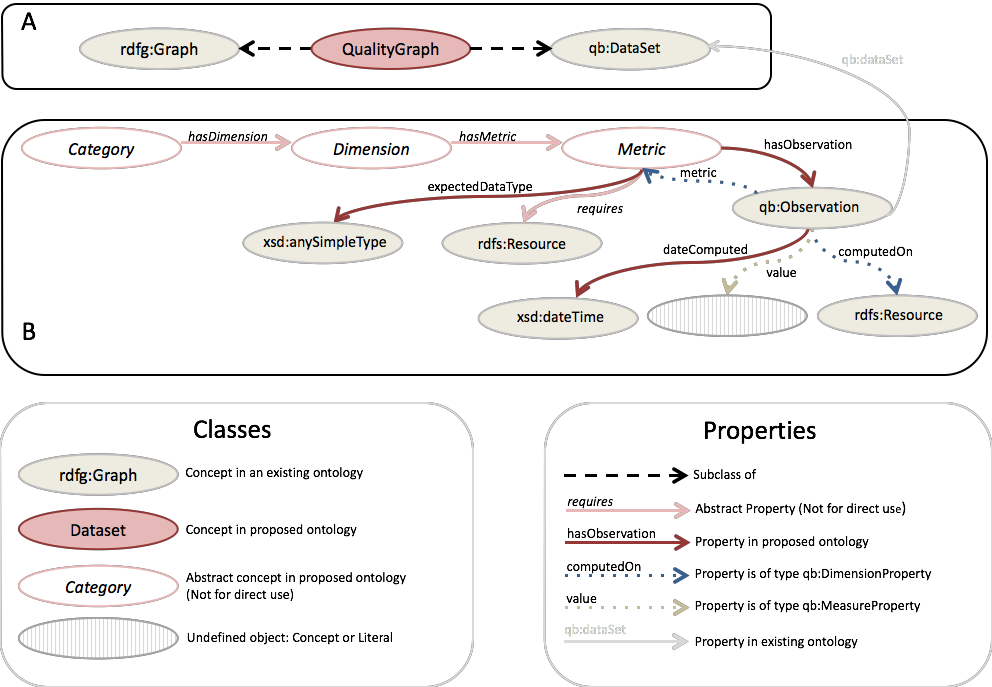
\includegraphics[width=.85\textwidth]{images/daq_extendedframework.png} 
\caption{The extended Dataset Quality Ontology (daQ)}
\label{fig:daqExtended}
\end{figure*}	

Using daQ, the quality metadata is intended to be stored in what we defined to be the \emph{Quality Graph}.
The latter concept is a subclass of \texttt{rdfg:Graph}~\cite{CBHS:NamedGraphs2005}.
This means that the quality metadata \todo{CL@JD: once more I'd rephrase to avoid the impression that \emph{we} are storing stuff.}is stored and managed in a separate named graph from the assessed dataset.
Named graphs are favoured due to
\begin{itemize}
\item the capability of separating the aggregated metadata with regard to computed quality metrics of a dataset from the dataset itself;
\item their use in the Semantic Web Publishing vocabulary~\cite{conf/semweb/CarrollBHS04} to allow named graphs to be digitally signed, thus ensuring trust in the computed metrics and defined named graph instance. Therefore, in principle each \texttt{daq:QualityGraph} can have the following triple \texttt{:myQualityGraph swp:assertedBy :myWarrant .}
\end{itemize}

The daQ ontology distinguishes between three layers of abstraction, based on the survey work by Zaveri et al.~\cite{Zaveri2012:LODQ}.
As shown in Figure~\ref{fig:daqExtended} Box B, a quality graph comprises of a number of different \emph{Categories}, which in turn possess a number of quality \emph{Dimensions}\footnote{In this deliverable we will refer to these as quality dimensions, in order to distinguish between the data cube dimensions}.
A quality dimension groups one or more computed quality \emph{Metrics}.
To formalise this, let $G$ represent the named Quality Graph (\texttt{daq:QualityGraph}), $C = \lbrace c_1, c_2,  \dots , c_x\rbrace$ is the set of all possible quality categories (\texttt{daq:Category}), $D = \lbrace d_1, d_2, \dots , d_y\rbrace$ is the set of all possible quality dimensions (\texttt{daq:Dimension}) and $M = \lbrace m_1, m_2, \dots , m_z\rbrace$ is the set of all possible quality metrics (\texttt{daq:Metric}); where $x,y,z\in \mathbb{N}$, then:

\newtheorem{Def1}{Definition}
\begin{Def1}
\label{def:daq_formalisation}
\begin{align*}
G \subseteq C, \\ 
C \subset D,\\
D \subset M; 
\end{align*}
\end{Def1}

Figure~\ref{fig:venn} shows this formalisation in a pictorial manner using Venn diagrams.

\begin{figure*}[tbph]
\center
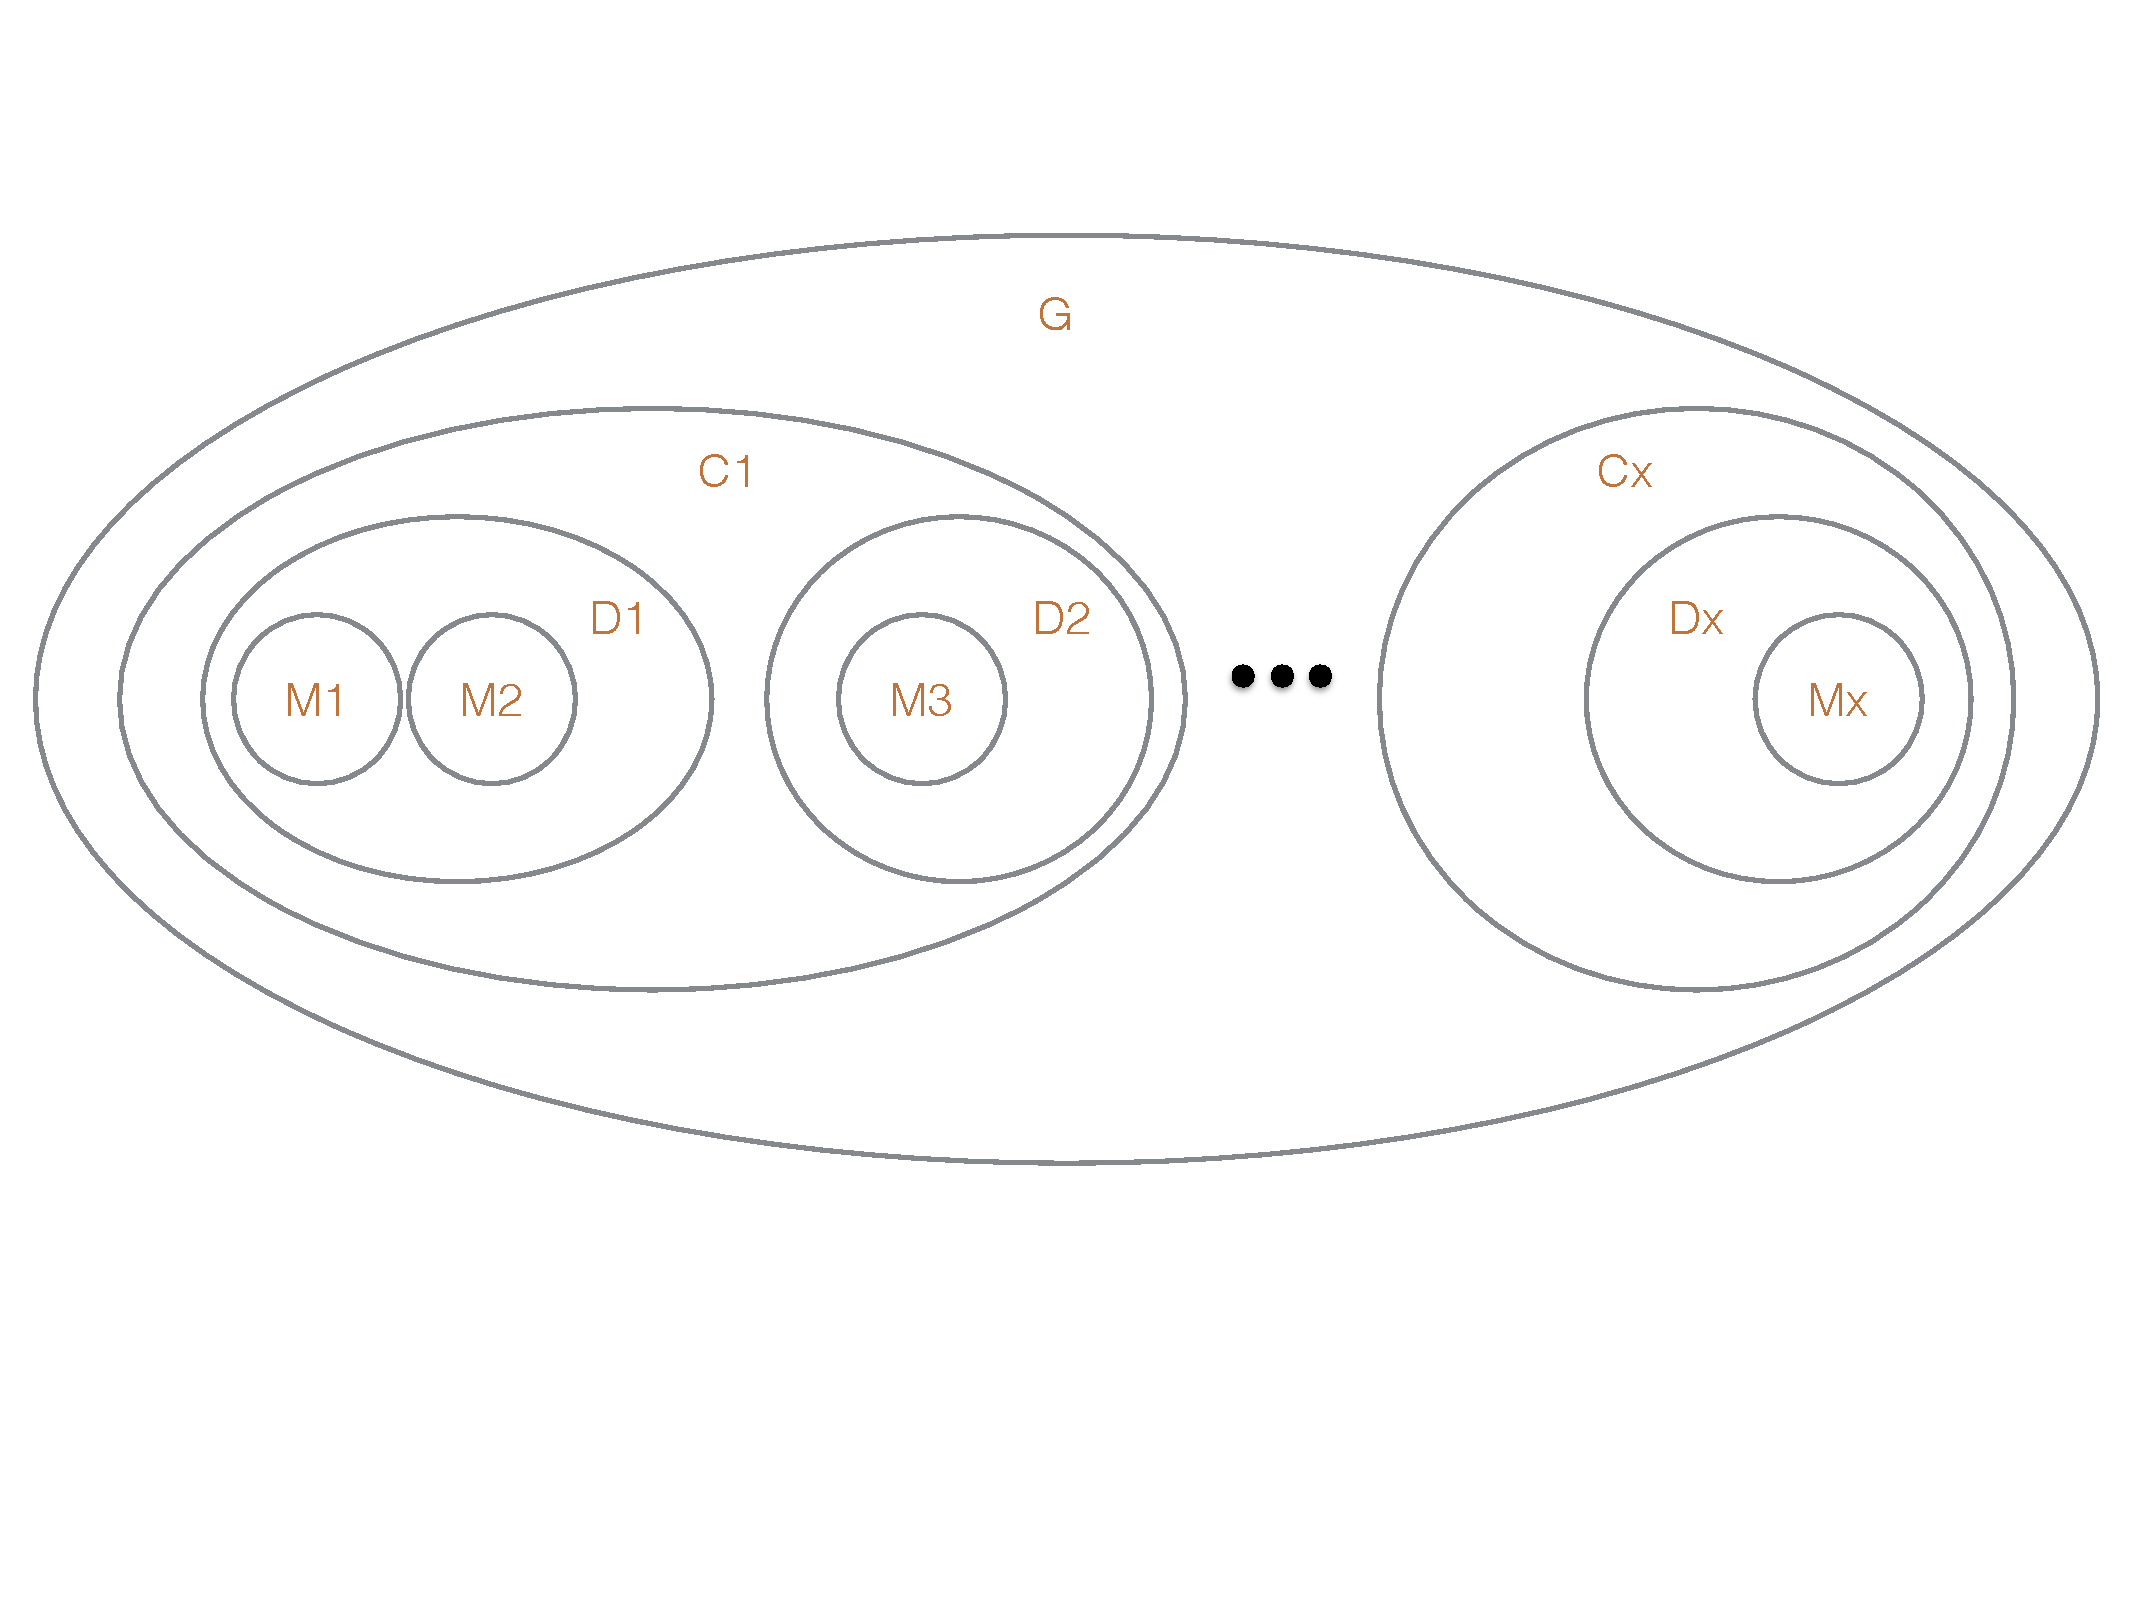
\includegraphics[scale=0.3]{images/venn.pdf} 
\caption{Venn Diagram depicting Definition~\ref{def:daq_formalisation} }
\label{fig:venn}
\end{figure*}

\subsubsection{Extending daQ for Multi-Dimension Representation and Statistical Evaluation}
The Data Cube Vocabulary~\cite{w3c:REC-vocab-data-cube-20140116} allows the representation of statistics about observations in a multidimensional attribute spaces. 
Multidimensional analysis of these observations, e.g.\ across the revision history of a dataset, would thus have required complex querying.
Extending daQ with the standardised Data Cube Vocabulary allows us to represent quality metadata of a dataset as a collection of \emph{Observations}, dimensions being the different quality metrics computed, the resources whose quality is assessed, revisions of these resources, and arbitrary further dimensions, such as the intended application scenario.
It also permits applying the wide range of tools that support data cubes to quality graphs, including the  CubeViz visualisation tool\footnote{\url{http://cubeviz.aksw.org}}.

A \emph{Quality Graph} is a special case of \texttt{qb:DataSet}, which allows us to represent a collection of quality observations complying to  a defined dimensional structure.
Each observation represents a quality metric measured out against a particular resource (e.g.\ a specific revision of a dataset).
daQ defines the structure of such observations by the \texttt{qb:DataStructureDefinition} shown in Listing~\ref{lst:dsd_def}.
\lstinputlisting[caption={The Data Structure Definition (Turtle Syntax)},label=lst:dsd_def, language=N3]{listings/dsd_def.trig}

The \texttt{daq:QualityGraph} also defines one restriction that controls the property \texttt{qb:structure} and its value to the mentioned definition, thus ensuring that all \emph{Quality Graph} instances make use of the standard definition.
Having a standard definition ensures that all \emph{Quality Graph}s conform to a common data structure definition, thus datasets with attached quality metadata can be compared.
Listing~\ref{lst:qg_def} describes the definition of \texttt{daq:QualityGraph}.
\lstinputlisting[caption={The Quality Graph Definition (Turtle Syntax)},label=lst:qg_def, language=N3]{listings/qg_def.trig}

\subsubsection{Abstract Classes and Properties}
This ontology framework (Figure~\ref{fig:daqExtended}) has three abstract classes/concepts (\texttt{daq:Category}, \texttt{daq:Dimension}, \texttt{daq:Metric}) and three abstract properties (\texttt{daq:hasDimension}, \texttt{daq:hasMetric}, \texttt{daq:requires}) which should not be used directly in a quality instance.
Instead these should be inherited as parent classes and properties for more specific quality metrics.
The abstract concepts (and their related properties) are described as follows:

\begin{description}
\item[daq:Category] represents the highest level of quality assessment.
  A category groups a number of dimensions.
\item[daq:Dimension $-$] In each dimension there is a number of metrics.
\item[daq:Metric] is the smallest unit of measuring a quality dimension.
  Each metric instance is linked to one or more observations. 
  Each observation has a value (\texttt{daq:value}), representing a score for the assessment of a quality attribute.
  This attribute is defined as a \texttt{qb:MeasureProperty}.
   Since this value is multi-typed (for example one metric might return true/false whilst another might require a floating point number), the value's \texttt{daq:hasValue} range is inherited by the actual metric's attribute defined by the property \texttt{daq:expectedDataType}.
  An observation must have the Dimension Properties (\texttt{qb:DimensionProperty}) \texttt{daq:computedOn} and \texttt{daq:metric}, which defines the assessed resource and the metric the mentioned resource was assessed by respectively.
  A metric might also require additional information (e.g.\ a gold standard dataset to compare with).
  Therefore, a \todo{CL@JD: to this maybe append ``i.e.\ an instance of a metric class''? - JD: agreed}instance of a metric representation can also define such properties using subproperties of the \texttt{daq:requires} abstract property.
  Another important attribute for any observation is the \todo{CL@JD: do you insist on this custom property, or can't we reuse dcterms:date? - JD: that should be changes, but i'll do it after the deliverable as it will take a lot of effort}\texttt{daq:dateComputed}, where it records the date of the observation's creation.
\end{description}

\subsubsection{Extending daQ for Custom/Specific Quality Metrics}
\label{sec:extendingDAQ}
The classes of the core daQ vocabulary can be extended by more specific and custom quality metrics. 
In order to use the daQ, one should define the quality metrics that characterise the ``fitness for use''~\cite{Juran1974:biblatex} in a particular domain.
We are currently in the process of defining the quality dimensions and metrics described in Deliverable 5.1.
\textbf{Extending} the daQ vocabulary means adding new quality protocols that inherit the abstract concepts (Category-Dimension-Metric).
Custom quality metrics do not need to be included in the daQ namespace itself; in fact, in accordance with LOD best practices, we recommend extenders to make them in their own namespaces.
In Figure~\ref{fig:ext_daq} we show an illustrative example of extending the daQ ontology (TBox) with a more specific quality attribute, i.e.\ the RDF Availability Metric as defined in~\cite{Zaveri2012:LODQ}, and an illustrative instance (ABox) of how it would be represented in a dataset.

The \texttt{Accessibility} concept is defined as an \texttt{rdfs:subClassOf} the abstract \texttt{daq:Category}.
This category has five quality dimensions, one of which is the \textit{Availability} dimension.
This is defined as an \texttt{rdfs:subClassOf} \texttt{daq:Dimension}.
Similarly, \textit{RDFAvailabilityMetric} is defined as an \texttt{rdfs:subClassOf} \texttt{daq:Metric}.
The specific properties \textit{hasAvailabilityDimension} and \textit{hasRDFAccessibilityMetric} (sub-properties of \texttt{daq:hasDimension} and \texttt{daq:hasMetric} respectively) are also defined (Figure~\ref{fig:ext_daq}).

\begin{figure*}[tbph]
\begin{center}
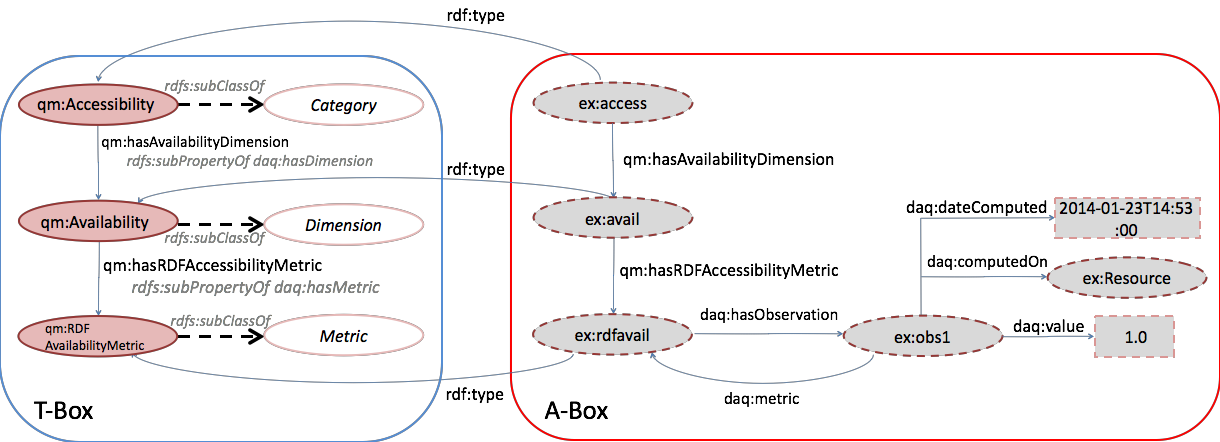
\includegraphics[width=\textwidth]{images/abox-tbox.png}
\caption{Extending the daQ Ontology – TBox and ABox}
\label{fig:ext_daq}
\end{center}
\end{figure*}

\subsubsection{A typical Quality Metadata Graph}
The excerpt listing in~\ref{lst:qg_example} show a typical quality graph metadata in a dataset.
\lstinputlisting[caption={A Quality Graph Excerpt (Turtle Syntax)},label=lst:qg_example, language=N3]{listings/lst1.trig}
The instance \emph{ex:qualityGraph1} is a named \texttt{daq:QualityGraph}.
The defined graph is automatically a \texttt{qb:DataSet}, and due to the restriction placed on the \texttt{daq:QualityGraph} (see Listing~\ref{lst:qg_def}), the value for the \texttt{qb:structure} property is defined as \texttt{daq:dsd} (see Listing~\ref{lst:dsd_def}).
In the named graph, instances for the \texttt{daq:Accessibility}, \texttt{daq:Availability}, \texttt{daq:EndPointAvailabilityMetric} and \texttt{daq:RDFAvailabilityMetric} are shown.
A metric instance has a number of observations.
Each of these observations specifies the metric value (\texttt{daq:value}), the resource the metric was computed on (\texttt{daq:computedOn} – here: different datasets, which are actually different revisions of one dataset), when it was computed (\texttt{daq:dateComputed}), the metric instance (\texttt{daq:metric}) and finally to what dataset the observation is defined in (\texttt{qb:dataSet}).

%%% Local Variables: 
%%% mode: latex
%%% TeX-master: "../../diachron-D5_2"
%%% End: 

%!TEX root = ../../diachron-D5_2.tex

\subsection{Design of the RESTful Quality API}
\label{sec:RestAPI} 
The RESTful API design and activity diagrams are explained in Deliverable 6.1, Section 6.1.7.
The only minor change is in the input parameters for the \texttt{\url{/diachron/compute_quality}} API call.
In Deliverable 6.1 we define the following two parameters:
\begin{description}
\item[Dataset -] An instance of a DIACHRON dataset URI;
\item[QualityReportRequired -] A boolean indicating whether a quality report is required.
\end{description}
The input parameter we introduce in this Deliverable is \textbf{MetricsConfiguration}.
This parameter is an object with a list of metrics (cf. Listing~\ref{lst:conf_metric}) in JSON-LD format, identifying the metrics required to be used for the dataset quality assessment.
Listing~\ref{lst:api_format} shows a sample input message format with the newly added parameter \textbf{MetricsConfiguration}.
\lstinputlisting[caption={API Call Input Message Format},label=lst:api_format, language=json]{listings/api_format.json} 
% relate to 6.1
%!TEX root = ../../diachron-D5_2.tex

\section{Tools and Libraries Used}
\label{sec:Libraries} 

In this section we discuss the main tools and libraries used in our solution to help us achieve our goal.

\subsection{OntoWiki}
\label{sec:OntoWiki}
OntoWiki\footnote{http://ontowiki.net/} is a tool providing support for agile, distributed knowledge engineering scenarios.
Based on semantic technologies, OntoWiki provides an easy to use control management system (CMS) that allows users to manage the knowledge base (RDF data) underlying the application.
OntoWiki is part of the LOD2 Stack, licensed under GPL and is open source.
The Quality Framework is currently based on top of OntoWiki.

\subsection{CubeViz}
\label{sec:CubeViz}
CubeViz\footnote{http://cubeviz.aksw.org} is an RDF DataCube browser and also an extension to OntoWiki.
This extension allows users to visually represent statistical data represented in RDF, specifically data which is modelled by the RDF DataCube vocabulary.
The Dataset Quality Vocabulary (daQ) is defined to use the mentioned RDF statistical vocabulary, thus CubeViz was a suitable extension to use to visualise statistical results about quality metadata.


\subsection{Apache Jena}
\label{sec:Jena}
Apache Jena\footnote{https://jena.apache.org} is an open source Java framework for building Semantic Web and Linked Data applications.
The framework is composed of different APIs interacting together to process RDF data. If you are new here, you might want to get started by following one of the tutorials.
Apache Jena is licensed under the Apache License, Version 2.0. 
This framework is the underlying technology used for the ``Quality Core Framework''.

\subsection{OpenRDF Sesame}
\label{sec:Sesame}
OpenRDF Sesame \footnote{http://www.openrdf.org/} is  a de-facto standard framework for processing RDF data. 
This includes parsers, storage solutions (RDF databases a.ka. triplestores), reasoning and querying, using the SPARQL query language. 
It offers a flexible and easy to use Java API that can be connected to all leading RDF storage solutions. 
The framework is licesed under BSD.


\subsection{Virtuoso}
\label{sec:Sesame}
Virtuoso \footnote{http://virtuoso.openlinksw.com/} is an innovative enterprise grade multi-model data server for agile enterprises and individuals.
It delivers an unrivaled  platform agnostic solution for data management, access, and integration.
Virtuoso is licensed under GNU General Public License (GPL) Version 2.
% mention all libraries used and their licences
%!TEX root = ../../diachron-D5_2.tex

\section{Assessment and Ranking Service}
\label{sec:RankingService} 

%!TEX root = ../../diachron-D5_2.tex

\subsection{Data Quality Assessment Process}
\label{sec:DQAssessment} 
In Deliverable 6.1 (Section 6.1.7.3), we described the assessment process in an activity diagram.
Since we need to cater for datasets modelled on the DIACHRON Data Model (cf. D1.3), the Stream Processor described in Section~\ref{sec:streamProcessor} requires some adaptation.
The DIACHRON data model is used as an underlying schema to store and query data from various heterogeneous sources using one standardised representation.
The schema features a number of key aspects that allow data to be traceable (indicating the provenance), reproducible, and overall enable the DIACHRON services (cf. D1.3).

Due to the nature of the heterogenous data that might originate from different models (e.g. triple-based, tuple-based, multidimensional etc.), the DIACHRON model is highly based on reified RDF.
This enables the description of resources as RDF statements (expanding a triple to a reification quad\footnote{\url{http://www.w3.org/TR/2004/REC-rdf-primer-20040210/#reification}}), recording further information such as provenance, attributes, relations and also changes.
Therefore, if we take for example the triple\footnote{This example does not follow the DIACHRON data model, but rather to illustrate a simple example of reification}:
\begin{lstlisting}[language=RDF]
ex:resourceSubject ex:property "value" .
\end{lstlisting}
it will be represented as a set of \texttt{rdf:Statement} triples:
\begin{lstlisting}[language=RDF]
ex:refiedResource rdf:type rdf:Statement .
ex:refiedResource rdf:subject ex:resourceSubject .
ex:refiedResource rdf:predicate ex:property .
ex:refiedResource rdf:object "value" .
\end{lstlisting}

In Section~\ref{sec:streamProcessor} we described how the \emph{Stream Processor} sequentially passes quads to the metrics in the \emph{Quality Assessment Layer}.
Although data based on the DIACHRON data model would be sufficient for the \emph{Stream Processor}, metric assessment will not give the desired results.
The main problem is that the most metrics would not just require the \emph{object} value, but would also require the \emph{subject} and the \emph{predicate}.
Therefore, DIACHRON resources have to be de-reified into RDF triple prior to them being passed to the metric.



% describe the process (similar to the activity diagram in 6.1). Mention the initialisation of metrics as required for each use case, and how the streaming process is done
%!TEX root = ../../diachron-D5_2.tex

\subsection{Data Quality Metrics}
\label{sec:DQMetrics} 

% describe what metrics have been implemented - separate in categories.
% Add more categories which metrics were implemented in, even if they are not important for ebi use case
% point to D5.1 for full details of the metrics


%Introduction
In this subsection we describe the metrics implemented as at the deliverable's deadline which are included in the first prototype of this service.
For this purpose, those metrics which are generally required by DIACHRON (\textbf{GEN}) and those specific by the pilot partners (Data Publica – \textbf{DP};  Scientific Pilot – \textbf{EBI}; cf. Deliverable 5.1~\cite[section 4]{diachron-d5.1}) were analysed and prioritised accordingly, also keeping in mind metrics required by the cleaning application discussed in Deliverable 3.2~\cite{diachron-d3.2}.
Some pilot partners required custom metrics (such as checking for \todo{CL@JD: I don't understand.  Do you mean a \emph{specific} property?}an additional property) to be implemented.
These will be identified with a $\star$.
Each implemented metric is expected to conform to the interface described in Section~\ref{sec:processingUnit}.

%~(required for: \textbf{GEN}, \textbf{DP}, \textbf{EBI})
%!TEX root = ../../../diachron-D5_2.tex

\subsubsection{Accessibility Category}
\label{sec:Accessibility} 

%Availability
\paragraph{Availability Dimension}~\\% dimension name 
Availability of a dataset is the extent to which data (or some portion of it) is present, obtainable and ready for use~\cite{Zaveri2012:LODQ}.

\paragraph{Dereferenceability Metric}~(required for: \textbf{GEN}, \textbf{EBI})~\\ %metric name
% background for the metric
HTTP URIs should be dereferencable, i.e. HTTP clients can retrieve the resources identified by the URI.
A typical web URI resource would return a \texttt{200 OK} code indicating that a request is successful and \texttt{4xx} or \texttt{5xx} if the request is unsuccessful. 
In Linked Data, a successful request should return a document (RDF) containing the description (triples) of the requested resource.
There are two possible ways which allow publishers make URIs dereferencable.
These are the \texttt{303} URIs and the \texttt{hash} URIs~\cite{W3C:CoolURIs}.
Yang et. al~\todo{CL: Where does this Dropbox source come from?  Google does not know this paper; has it never been published?  Can we cite something else?}\cite{Yang2011} describes a mechanism to identify the dereferenceability process of linked data resource.
% short description
\begin{mdframed}[style=metricdefinition]
\emph{Calculates the number of valid redirects (303) or hashed links according to LOD Principles.}
\end{mdframed}

% pseudocode
The dereferenceability metric (listing~\ref{lst:deref}) counts the number of valid dereferenceable URI resources found in the subject (?s) and object (?o) position of a triple. The \texttt{isDereferenceable(resource)} method uses the rules defined in~\todo{CL: please add to bib}\cite{Yang2011}.
\begin{algorithm}
\caption{Dereferenceability Algorithm}\label{lst:deref}
\begin{algorithmic}[1]
\Procedure{init}{}
\State totalTriples = 0 ;
\State deref = 0 ;
\EndProcedure

\Procedure{Dereference}{$\langle?s,?p,?o,?g\rangle$}
\If {(isURI(?s)) \&\& (isDereferenceable(?s))} deref++ ; \EndIf

\If {(isURI(?o)) \&\& (isDereferenceable(?o))} deref++ ; \EndIf
\State totalTriples++;
\EndProcedure
\end{algorithmic}
\end{algorithm}
% metric value, range and rating
The metric returns a ratio of the number of dereferenced URIs (deref) against the total number of triples in a dataset (totalTriples). The expected range is $[0,\ldots,1]$, where 0 is the worst rating and 1 is the best rating.

\paragraph{RDF Accessibility Metric}~(required for: \textbf{EBI})~\\
A data source should be available as a LOD format (e.g. RDF) dump which can be downloaded by a consumer.
This dump should be stated in the dataset and accessible under the given URI.

\begin{mdframed}[style=metricdefinition]
\emph{Check if data dumps (void:dataDump) exists and are reachable and parsable.}
\end{mdframed}

\begin{algorithm}
\caption{RDF Accessibility Algorithm}\label{lst:deref}
\begin{algorithmic}[1]
\Procedure{init}{}
\State lodDumps = 0 ;
\State accessibleLodDumps = 0 ;
\EndProcedure

\Procedure{RDFAccessibility}{$\langle?s,?p,?o,?g\rangle$}
\If {?p is void:dataDump} lodDumps++ ; \EndIf
\If {isAccessible(?o)} accessibleLodDumps++ ; \EndIf
\EndProcedure
\end{algorithmic}
\end{algorithm}

The metric returns a ratio between the number of defined LOD data dumps (lodDumps) and the total number of accessible data dumps (accessibleLodDumps). 
The expected range is $[0,\ldots,1]$, where 0 is the worst rating and 1 is the best rating. If no data dump is found, then the metric would return 0 and thus the dataset fails this metric.

\paragraph{SPARQL Accessibility Metric}~(required for: \textbf{EBI})~\\
This metric follows the previous (RDF Accessibility Metric), where a dataset is assessed to check if a SPARQL endpoint is defined.

\begin{mdframed}[style=metricdefinition]
\emph{Check if a SPARQL endpoint (matching void:sparqlEndpoint) is available and returns a result.}
\end{mdframed}

\begin{algorithm}
\caption{SPARQL Accessibility Algorithm}\label{lst:deref}
\begin{algorithmic}[1]
\Procedure{init}{}
\State endPoints = 0 ;
\State accessibleEndPoints = 0 ;
\EndProcedure

\Procedure{SPARQLAccessibility}{$\langle?s,?p,?o,?g\rangle$}
\If {?p is void:sparqlEndpoint} 
\State endPoints++ ; 
\State query ?o ;
\If {returnResult(?o)} accessibleEndPoints++ ; \EndIf
\EndIf
\EndProcedure
\end{algorithmic}
\end{algorithm}

The metric returns a ratio between the number of defined SPARQL endpoints (endPoints) and the total number of accessible SPARQL endpoints (accessibleEndPoints). 
The expected range is $[0,\ldots,1]$, where 0 is the worst rating and 1 is the best rating. If no endpoint is defined, then the metric would return 0 and the dataset fails this metric

\paragraph{Performance Dimension}~\\ % dimension name 
In a broad sense, performance refers to the ability to get access to the Linked Data source efficiently, without causing any major delays in the client application when querying the data. It constitutes a highly important quality feature, as low performance can seriously affect the ability of clients to access the data (availability) and its usability. There are a variety of factors that can have an effect on performance, such as networking issues, server configurations and usage of complex RDF features.

\paragraph{Low Latency Metric}~(required for: \textbf{EBI}) ~\\ %metric name
% background for the metric
Latency is a measure of the response-time of a data source, defined by Bizer as \cite{Bizer2008:PhDThesis:biblatex}: ``the delay between submission of a request by the user and reception of the response from the system''. Achieving low latency should be one of the main goals, from a performance perspective, of a Linked Data service, as it negatively affects the responsiveness of client applications and hence, their ability to provide the user with timely information.
% short description
\begin{mdframed}[style=metricdefinition]
\emph{Estimates the efficiency with which a system can bind to the dataset, by measuring the delay between the submission of a request  and the reception of the corresponding response, sent back from the system.}
\end{mdframed}

% pseudocode
As shown in algorithm~\ref{alg:lowLatency}, the implementation of this metric consists in figuring out the URI of the dataset from which the triples were obtained, to afterwards send several HTTP requests to their source. The respective response times are then averaged to obtain a measure of the latency. Note that this metric refers to the resource itself, not to its contents.
\begin{algorithm}
\caption{Low Latency Algorithm} \label{alg:lowLatency}
\begin{algorithmic}[1]
\Procedure{init}{}
\State totalDelay = $-1$;
\State requestsToSend = 2;
\EndProcedure
\Procedure{compute}{$\langle?s,?p,?o,?g\rangle$}
\If {isDataSetURI(?s)} 
\State startTimer();
\For{$i=0$ to requestsToSend}
\State sendSynchronousRequestTo(?s);
\EndFor
\State timeElapsedSinceStart = stopTimer();
\State totalDelay += timeElapsedSinceStart;
\EndIf
\Return{totalDelay / requestsToSend;}
\EndProcedure
\end{algorithmic}
\end{algorithm}
% metric value, range and rating
The result of the metric is a real number in the range $[1, +\infty)$, as it represents the average time (in  milliseconds) elapsed between the issuing of the request and the reception of its response. The lower the value, the better, as it represents how long does it take to get access to the dataset.

% end-of Low Latency metric

\paragraph{High Throughput Metric}~(required for: \textbf{EBI}) ~\\ %metric name
% background for the metric
As latency, throughput is a determining factor when assessing the performance of a data source, since it measures the rate at which a service can provide data as response to client requests. If a service is unable to handle a reasonable amount of data requests, in a timely fashion, its usability and the performance of clients themselves could be severely affected. Therefore, it is desirable that the Linked Data source is able to properly respond to as many requests as possible during a limited period of time.
% short description
\begin{mdframed}[style=metricdefinition]
\emph{Measures the efficiency with which a system can access the dataset, as the average number of requests responded by the service hosting it, per second.}
\end{mdframed}

% pseudocode
The throughput of the resource is measured by sequentially sending it a fixed number of requests and by totalling the response time of all of them (time elapsed between the sending of the request and the reception of the response). Afterwards, the total number of requests is divided by their total response time. Algorithm \ref{alg:highThroughput} provides additional details.
\begin{algorithm}
\caption{High Throughput Algorithm} \label{alg:highThroughput}
\begin{algorithmic}[1]
\Procedure{init}{}
\State totalDelay = $-1$;
\State requestsToSend = 3;
\EndProcedure
\Procedure{compute}{$\langle?s,?p,?o,?g\rangle$}
\If {isDataSetURI(?s)} 
\State startTimer();
\For{$i=0$ to requestsToSend}
\State sendSynchronousRequestTo(?s);
\EndFor
\State timeElapsedSinceStart = stopTimer();
\State totalDelay += timeElapsedSinceStart;
\EndIf
\Return{requestsToSend / totalDelay;}
\EndProcedure
\end{algorithmic}
\end{algorithm}
% metric value, range and rating
The value of the metric is in the range $[1 +\infty)$ and represents the average number of requests successfully served by the resource's host per millisecond. The higher the value, the better, as it represents the number of requests per second, that the data-source is able to serve.

% end-of High Throughput Metric


\paragraph{Scalability of a Data Source Metric}~(required for: \textbf{EBI}) ~\\ %metric name
% background for the metric
A Linked Data resource that scales well will be able to handle a high, growing amount of requests in an acceptable period of time. This capability will prevent the service from becoming overloaded and hence unresponsive under heavy demand. Thus, scalability helps assure  that the data source will be accessible at any time and is an important quality factor regarding performance.
% short description
\begin{mdframed}[style=metricdefinition]
\emph{Measures the scalability of the data source, by determining whether the average response time of several requests (ten by default), sent simultaneously, is approximately equal to the response time of a single request \cite{Flemming2008}.}
\end{mdframed}

% pseudocode
All the requests whose response times (delays) are to be averaged, are sent simultaneously (in parallel), in order to increase the workload on the server. After all these parallel requests have been responded, their respective delays are averaged. Subsequently, a single request is sent, and its delay is compared with the average delay of the parallel requests. This process is outlined in algorithm \ref{alg:scalabilityData}.
\begin{algorithm}
\caption{Scalability of a Data Source Algorithm} \label{alg:scalabilityData}
\begin{algorithmic}[1]
\Procedure{init}{}
\State numSimultaneousRequests = 10;
\State totalDelaySimultaneousReqs = $-1$;
\State totalDelaySingleReq = $-1$;
\EndProcedure
\Procedure{compute}{$\langle?s,?p,?o,?g\rangle$}
\If {isDataSetURI(?s)} 
\State startTimer();
\State sendAsynchronousRequestsTo(?s, numSimultaneousRequests);
\State totalDelaySimultaneousReqs = stopTimer();
\State startTimer();
\State sendSynchronousRequestTo(?s);
\State totalDelaySingleReq = stopTimer();
\EndIf
\Return{(totalDelaySimultaneousReqs / numSimultaneousRequests) - totalDelaySingleReq;}
\EndProcedure
\end{algorithmic}
\end{algorithm}
% metric value, range and rating
The value of the metric is in the range $[0, +\infty)$ it consist of the difference in milliseconds, between the average response time of the data source, when exposed to several, simultaneous requests and the response time of a single, isolated request. The lower the value, the better. Higher values suggest poor scalability of the data source, as they mean that it gets overwhelmed by multiple, simultaneous requests.

% end-of Scalability of a Data Source Metric


\paragraph{Security Dimension}~\\ % dimension name
Security refers to the capability of restricting access to the data and of guaranteeing that communication between the Linked Data source and its consumers is confidential and protected against tampering, as defined by Flemming in \cite{Flemming2008}. Conspicuously, the importance of security strongly depends on the nature of the data contained in the resource and also on the application domain, up to the extent that this dimension becomes a critical quality feature when dealing with sensitive information.


\paragraph{HTTPS Data Access Metric~$\star$}~(required for: \textbf{EBI}) ~\\ %metric name
% background for the metric
A dataset hosted under a properly configured HTTPS service ensures that communications with its clients are secured by the SSL/TLS protocol. This prevents unauthorised parties from intercepting and getting access to sensitive information and from impersonating the legitimate data provider. Offering a secure connection through HTTPS, has a positive effect on the accessibility of Linked Data resources containing sensitive data, as consumers could otherwise be reluctant to even consult them.

% short description
\begin{mdframed}[style=metricdefinition]
\emph{Verifies whether the authenticity of the data source is assured and the communication channel is confidential, by verifying that access to it is carried out through a sound, HTTPS connection.}
\end{mdframed}

% pseudocode
As shown in algorithm \ref{alg:httpsDataAccess}, once the URI of the dataset has been determined, it is tested to correspond to the HTTPS protocol, if so, an HTTPS connection is attempted to be established. If no errors occur, and a request is successfully sent through such connection, the data source is considered to be safe.
\begin{algorithm}
\caption{HTTPS Data Access Algorithm} \label{alg:httpsDataAccess}
\begin{algorithmic}[1]
\Procedure{init}{}
\State httpsConnectionSucceeded = 0;
\EndProcedure
\Procedure{compute}{$\langle?s,?p,?o,?g\rangle$}
\If {isDataSetURI(?s) \&\& isHTTPS(?s)} 
\State httpsConnectionSucceeded = sendTestRequestHTTPS(?s);
\EndIf
\Return{httpsConnectionSucceeded;}
\EndProcedure
\end{algorithmic}
\end{algorithm}
% metric value, range and rating
The value of the metric is binary: it will return 1 if an HTTPS connection was successfully established with the data source and 0 otherwise. Thus, a value of 1 corresponds to the best possible quality rating.

% end-of HTTPS Data Access Metric

\paragraph{Licensing Dimension}~\\ % dimension name
In an open data world, such as that of Linked Open Data, it is important to be aware of the terms under which data sources can be accessed and used. In order to prevent any inconveniences and to assure that information is distributed according to the publisher's rules, consumers should make sure that the datasets they use are available under clear legal terms.

\paragraph{Machine-readable Indication of a License Metric} ~\\ %metric name
% background for the metric
As stated by Hogan et al. \cite{Hogan2012:LDC}, each dataset should contain a license specifying how the content can be used. Such a license can be machine-readable, if provided by means of any of the several properties defined for that purpose. Having access to the license this way, enables customers to automatically check that the permissions granted upon the data have been specified and hence, leverages accessibility to the dataset.
The dataset is assessed by checking if triples contain any of the following predicates:
\begin{itemize}
\item \url{http://purl.org/dc/terms/license}
\item \url{http://purl.org/dc/terms/accessRights}
\item \url{http://purl.org/dc/terms/rights}
\item \url{http://purl.org/dc/elements/1.1/rights}
\item \url{http://www.w3.org/1999/xhtml/vocab#license}
\item \url{http://creativecommons.org/ns#license}
\end{itemize}

% short description
\begin{mdframed}[style=metricdefinition]
\emph{Checks whether consumers of the dataset are explicitly granted permission to re-use it, under defined conditions, by annotating the resource with a machine-readable indication of the license.}
\end{mdframed}

% pseudocode
Algorithm \ref{alg:machineReadLicense} details how the metric is computed. Firstly, the URI of the dataset is determined from the triples as they are processed. Having the dataset's URI, the triples providing licensing information about it can be looked for.
\begin{algorithm}
\caption{Machine-readable Indication of a License Algorithm} \label{alg:machineReadLicense}
\begin{algorithmic}[1]
\Procedure{init}{}
\State dataSetURI = null;
\State hasMachineReadLicense = 0;
\EndProcedure
\Procedure{compute}{$\langle?s,?p,?o,?g\rangle$}
\If {isDataSetURI(?s)} 
\State dataSetURI = ?s;
\EndIf
\If {isLicensingProperty(?p) \&\& ?s == dataSetURI} 
\State hasMachineReadLicense = 1;
\EndIf ~\\
\Return{hasMachineReadLicense;}
\EndProcedure
\end{algorithmic}
\end{algorithm}
% metric value, range and rating
The value of the metric is binary: a value of 1 indicates that machine-readable licensing information was found as part of the dataset, whereas 0 indicates that it was not. Therefore, 1 elicits a higher quality ranking.

% end-of Machine-readable Indication of a License Metric


%%%%%%% Bibliography
% Yang2011 : https://dl.dropboxusercontent.com/u/4138729/paper/dereference_iswc2011.pdf

%%% Local Variables: 
%%% mode: latex
%%% TeX-master: "../../../diachron-D5_2"
%%% End: 

%!TEX root = ../../../diachron-D5_2.tex

%~(required for: \textbf{GEN}, \textbf{DP}, \textbf{EBI})
\subsubsection{Intrinsic Category}
\label{sec:Intrinsic}
The intrinsic category metrics are independent of the user's context.
They reflect whether information presented in data correctly represent the real world and whether information is logically consistent itself.

\paragraph{Accuracy Dimension}~\\% dimension name 
Accuracy dimension metrics reflect the degree of correctness and precision with which the given dataset represent the real world facts.

\paragraph{Malformed Datatype Literals Metric}~(required for: \textbf{GEN}, \textbf{DP}, \textbf{EBI})~\\ %metric name
Literals in RDF are values, plain or typed, containing a textual string (eg. ``13''\string^\string^xsd:int).
It is common problem in LOD datasets that the literal value does not match its describing data type. 
The Malformed Datatype Literals metric intends to check this inconsistency.
The algorithm \ref{lst:malformedLiterals} describes the metric computation in more details.

\begin{mdframed}[style=metricdefinition]
\emph{Calculates the ratio of invalid typed literals against all literals}
\end{mdframed}

\begin{algorithm}
\caption{Malformed Datatype Literals Algorithm}\label{lst:malformedLiterals}
\begin{algorithmic}[1]
\Procedure{init}{}
\State totalLiterals = 0 ;
\State malformedLiterals = 0 ;
\EndProcedure

\Procedure{compute}{$\langle?s,?p,?o,?g\rangle$}
\If {(isLiteral(?o))} totalLiterals++ ;
\If {(isTypedLiteral(?o)) \&\& (!hasValidDatatype(?o))} malformedLiterals++ ; \EndIf
 \EndIf
\EndProcedure
\end{algorithmic}
\end{algorithm}

Only the typed literals are considered by the metric. 
The metric values vary in the interval $[0,\ldots,1]$, where the 0 indicates the best quality.\todo{CL@JD: I think this is a good candidate for making the value ranges more uniform.  As with many other metrics we should say 0 is worst.  Can we change it now (and then in the implementation soon)?}

\paragraph{Literals Incompatible with Datatype Range Metric}~(required for: \textbf{GEN}, \textbf{DP}, \textbf{EBI})~\\
Similar to the previously described metric, this verifies the correctness of literals regarding their datatype. 
By correctness, we mean that the data type attached to the literal is different than the one specified by the range of the used property in the ontology.
Algorithm~\ref{alg:dataRange} describes this metric.
\begin{mdframed}[style=metricdefinition]
\emph{Calculates the ratio of incorrectly defined literals against all literals in the dataset.}
\end{mdframed}

\begin{algorithm}
\caption{Literals Incompatible with datatype range}\label{alg:dataRange}
\begin{algorithmic}[1]
\Procedure{init}{}
\State totalLiterals = 0
\State incompatibleLiterals = 0
\EndProcedure
\Procedure{compute}{$\langle?s,?p,?o,?g\rangle$}
\If {isLiteral(?o)} totalLiterals++ ;
\If {hasRange(?p) \&\& (literalDatatype(?o)!=rangeDatatype(?p)) } imcompartibleLiterals++; 
\EndIf
\EndIf
\EndProcedure
\end{algorithmic}
\end{algorithm}

Only the literals referring by the property with the range characteristic are considered by the metric. 
The metric values vary in the interval $[0, 1]$, where  0 indicates the best quality\todo{CL@JD: once more I'd define 0 = worst}.

\paragraph{Defined Ontology Author Metric$\star$}~(required for: \textbf{EBI})~\\ 
This metric is required of the Scientific Linked Data scenario as defined in Deliverable 5.1.
Imported ontologies should have common metadata which includes the definition of an author.

\begin{mdframed}[style=metricdefinition]
\emph{Checks whether the creator \texttt{efo:creator} is defined in the ontology}
\end{mdframed}

\begin{algorithm}
\caption{Defined Ontology Author Algorithm}
\begin{algorithmic}[1]
\Procedure{compute}{$\langle?s,?p,?o,?g\rangle$}
\If {?o is owl:Ontology} ontologyList.add(?s); \EndIf
\If {?p is efo:creator \&\& ?s in ontologyList} definedCreator = 1 ; \EndIf
\EndProcedure
\end{algorithmic}
\end{algorithm}

The metric will return a 1 (best rating) if the creator of the ontology is defined or 0 if otherwise.

\paragraph{POBO Definition Usage Metric$\star$}~(required for: \textbf{EBI})~\\ 
This metric is required of the Scientific Linked Data scenario as defined in Deliverable 5.1.
For this use case, it is required to check that each ontology class has a corresponding human readable definition.

\begin{mdframed}[style=metricdefinition]
\emph{Provides a measure for an ontology to check the usage of \texttt{pobo:def} in defined classes}
\end{mdframed}

\begin{algorithm}
\caption{POBO Definition Usage Algorithm}
\begin{algorithmic}[1]
\Procedure{compute}{$\langle?s,?p,?o,?g\rangle$}
\If {?o is owl:Class} ontologyClassList.add(?s); \EndIf
\If {?p is pobo:def \&\& ?s in ontologyClassList} 
\State definitionHashMap.put(?s,?o);
\EndIf
\EndProcedure
\end{algorithmic}
\end{algorithm}

The metric will return a ratio of the number of classes without definitions against the total number defined classes. The expected range is $[0,\ldots,1]$, where 0 is the worst rating and 1 is the best rating

\paragraph{Synonym Usage Metric$\star$}~(required for: \textbf{EBI})~\\ 
This metric is required of the Scientific Linked Data scenario as defined in Deliverable 5.1.
Scientific terms usually have a number of synonyms.
Each ontology term should have at least one \todo{CL: Do we need the word ``more''?}more synonym, thus in this metric we check if defined terms have a synonym attached to their description.

\begin{mdframed}[style=metricdefinition]
\emph{Measures the number of classes which has a synonym \texttt{efo:alternative\_term} described}
\end{mdframed}

\begin{algorithm}
\caption{Synonym Usage Algorithm}
\begin{algorithmic}[1]
\Procedure{compute}{$\langle?s,?p,?o,?g\rangle$}
\If {?o is owl:Class} ontologyClassList.add(?s); \EndIf
\If {?p is efo:alternative\_term \&\& ?s in ontologyClassList} 
\State synonomHashMap.put(?s,?o);
\EndIf
\EndProcedure
\end{algorithmic}
\end{algorithm}

The metric will return a ratio of the number of classes without synonyms against the total number defined classes. The expected range is $[0,\ldots,1]$, where 0 is the worst rating and 1 is the best rating

\paragraph{Consistency Dimension}~\\ 
Consistency metrics intend to identify any kinds of contradictions in data.
%\paragraph{Entities As Members of Disjoint Classes}~\\
\paragraph{Homogeneous Datatypes}~(required for: \textbf{GEN}, \textbf{DP}, \textbf{EBI})~\\
In some cases, the range of a property in a vocabulary is either (i) not defined; or (ii) given an open/generic type (such as \texttt{rdfs:Literal}).
This could cause inconsistencies in a dataset since values defined by the same property can be used with literals of different datatypes.
In contrast to the \emph{Malformed Literal} metric and \emph{Incompatible Datatype} metric, this metric deals  with the object in a triple where its property has an undefined/open range. 
The metric computation therefore contains the following steps:
\begin{itemize}
\item Count the frequency of different datatypes occurring with a particular predicates.
\item Identify the properties corresponding to heterogeneous datatype literals.
\end{itemize}

\begin{mdframed}[style=metricdefinition]
\emph{Calculates the ratio of inconsistent object values in a dataset}
\end{mdframed}

% pseudocode
\begin{algorithm}
\caption{Homogeneous Datatypes}\label{lst:heterogeneous}
\begin{algorithmic}[1]
\Procedure{init}{}
\State totalProperties = 0;
\State heterogeneousDatatypeProperties = 0
\State  propertyMap = map(Property, List<Datatype>)
\EndProcedure
\Procedure{analyzeProperties}{$\langle?s,?p,?o,?g\rangle$}
\If {isLiteral(?o)}  propertyMap.put(?p, Set.add.datatypeOf(?o)); \EndIf
\EndProcedure
\Procedure{compute}{}
\ForAll {Properties in propertyMap}
\If {size(Set$\langle$Datatype$\rangle$) $\rangle$ 1 } heterogeneousDatatypeProperties++; 
\EndIf
totalProperties ++;
\EndFor
\EndProcedure
\end{algorithmic}
\end{algorithm}

The metric values vary between $[0,\ldots,1]$, when the 0 indicates no properties containing heterogeneous datatype literals\todo{CL: let's say 0 = worst}.
  
\paragraph{Misplaced Classes or Properties}~\\
In some cases a URI that occurs in the predicate position of a triple is defined in the corresponding vocabulary as a class, or a contrariwise a URI in the subject or object position is a defined property.
These kind of inconsistencies make machine interpretation of the data more complex.
More details about the metric computation are shown in algorithm \ref{lst:misplacedCl}.

\begin{mdframed}[style=metricdefinition]
\emph{Identifies the percentage of misplaced classes and properties in a dataset.}
\end{mdframed}

\begin{algorithm}
\caption{Misplaced Classes or Properties Metric Algorithm}\label{lst:misplacedCl}
\begin{algorithmic}[1]
\Procedure{init}{}
\State totalClassesAndProperties = 0 ;
\State misplacedClasses = 0 ;
\State misplacedProperties = 0 ;
\EndProcedure

\Procedure{compute}{$\langle?s,?p,?o,?g\rangle$}
\If {isURI(?p)} totalClassesAndProperties++ ;\EndIf 
\If {!isProperty(?p)} misplacedProperties++ ; \EndIf 

\If {isURI(?o)} totalClassesAndProperties++; \EndIf  
\If {!isClass(?o)} misplacedClasses++ ; \EndIf 
\Return{(misplacedClasses+misplacedProperties) / totalClassesAndProperties}
\EndProcedure
\end{algorithmic}
\end{algorithm}

The metric values vary between  $[0,\ldots,1]$, where  the 0 indicates the best quality.

\paragraph{Misused OWL Datatype or Object Properties}~(required for: \textbf{EBI})~\\
The OWL language defines additional characteristics to some properties. 
A property can be either an instance of the \textit{owl:ObjectProperty} or \textit{owl:DatatypeProperty} class.
A datatype property relates some resource to a literal value, while an object property describes a relation between two resources.
Wrong usage of the datatype and object properties indicates inconsistencies in the data.
The following algorithm  \ref{lst:misusedCl} presents more details about how the metric is computed.

\begin{mdframed}[style=metricdefinition]
\emph{Ratio of misused datatype and object properties to all properties}
\end{mdframed}

\begin{algorithm}
\caption{Misused OWL Datatype or Object Properties Metric Algorithm} \label{lst:misusedCl}
\begin{algorithmic}[1]
\Procedure{init}{}
\State totalProperties = 0 ;
\State misusedObjectProperties = 0 ;
\State misusedDatatypeProperties = 0 ;
\EndProcedure

\Procedure{compute}{$\langle?s,?p,?o,?g\rangle$}
\If {isURI(?p)} totalProperties++ ;\EndIf 
\If {isDatatypeProperty(?p) \&\& isURI(?o)} misusedDatatypeProperties++ ; \EndIf 
\If {isObjectProperty(?p) \&\& isLiteral(?o)} misusedObjectProperties++ ; \EndIf 
\EndProcedure
\end{algorithmic}
\end{algorithm}

The metric gives a value between $[0,\ldots,1]$, where  the 0 indicates the best quality.

\paragraph{Obsolete Concepts in Ontology$\star$}~(required for: \textbf{EBI})~\\
TODO TODO

\paragraph{Ontology Hijacking}~(required for: \textbf{EBI})~\\
\emph{Ontology Hijacking} was introduced by Hogan et. al~\cite{Hogan08} and is defined as ``the contribution of statements about classes and/or properties in a non-authoritative source such that reasoning on those classes and/or properties is affected''. 
In other words ontology hijacking refers to cases where external concepts are redefined in a local ontology.
Defining new super classes or properties of third-party classes or properties is an example for this problem, e.g. declaring \textit{rdfs:subPropertyOf} which is defined as a property, to be a \textit{rdfs:Class}. 
%The challenging question is how to define authoritative source.
%We assume the ontologies/vocabularies published according to the best-practices as authoritative, while all other vocabularies as third parties documents.
%More formal, a concept (class or property) is authoritative if it's not a blank node and if the corresponding vocabulary is retrievable.
To identify hijacked terms  we define a set of properties $P$:
\begin{itemize}
\item\textit{rdf:type}, \item\textit{rdf:domain}, \item\textit{rdf:range}, \item\textit{rdfs:subClassOf}, \item\textit{rdfs:subPropertyOf}\item\textit{owl:equivalentClass}, \item\textit{owl:equivalentProperty}, \item\textit{owl:inverseOf}, \item\textit{owl:onProperty}, \item\textit{owl:hasValue}, \item\textit{owl:someValuesFrom}, \item\textit{owl:allValuesFrom}, \item\textit{owl:intersectionOf}, \item\textit{owl:unionOf}, \item\textit{owl:maxCardinality}, \item\textit{owl:cardinality}, \item\textit{owl:oneOf};
\end{itemize}
and a set of classes $C$: 
\begin{itemize}
\item\textit{owl:FunctionalProperty}, \item\textit{owl:InverseFunctionalProperty}, \item\textit{owl:TransitiveProperty}, \item\textit{owl:SymmetricProperty}.
\end{itemize}
Metric check the two following cases:
\begin{itemize}
\item Classes in \textbf{C} appear in a position other than the object of a \textit{rdf:type} triple. 
\item Properties in \textbf{P} appear in a position other than the predicate position.
\end{itemize}

\todo{CL: we actually only check for redefinition, don't we?  Without an OWL reasoner we can't check whether such a redefinition breaks consistency.}
\begin{mdframed}[style=metricdefinition]
\emph{Checks for the re-definition of defined concepts breaking the consistency.}
\end{mdframed}

\begin{algorithm}
\caption{Ontology Hijacking Algorithm}\label{lst:undefCl}
\begin{algorithmic}[1]
\Procedure{init}{}
\State hijackedTriples = 0 ;
\State totalTriples = 0 ;
\EndProcedure

\Procedure{compute}{$\langle?s,?p,?o,?g\rangle$}
\If {(($?s \in \textbf{C}$) or ($?o \in \textbf{C}$))\&\& ($?p== \textit{rdf:type}$)} hijackedTriples++ ;\EndIf
\If {($?p \in \textbf{P}$) \&\& isAuthority(?s) \&\& !isAuthority(?o)} hijackedTriples++; \EndIf
\EndProcedure
\end{algorithmic}
\end{algorithm}

\paragraph{Undefined Classes Metric}~(required for: \textbf{GEN})~\\ 
A class is defined in a vocabulary or dataset by the predicate \texttt{rdf:type} and an object value of \texttt{rdf:Class} or \texttt{owl:Class}.
In the case when LOD dataset defines its own vocabulary the following predicates indicate that the object must be a defined class:  \texttt{rdfs:domain}, \texttt{rdfs:range}, \texttt{rdfs:subClassOf}, \texttt{owl:allValuesFrom}, \texttt{owl:someValuesFrom}, \texttt{owl:equivalentClass}, \texttt{owl:complementOf}, \texttt{owl:onClass}, \texttt{owl:disjointWith}.
%'Being defined' means that the term is defined either in some external ontology or at an earlier position in the given dataset. 
%According to Hogan~\todo{CL: please add to bib}\cite{hogan2010} to the most used undefined classes belong \texttt{foaf:UserGroup}, \texttt{rss:item}, \texttt{linkedct:link}, \texttt{politico:Term} .
%The probability for undefined class in the subject position is very low, because the subject of a quad never references classes or properties in external vocabularies.
%Therefore they is no need to analyze the subject for this metric.
%For the most LOD datasets is sufficient to check object by the predicate \texttt{rdf:type}. 
The undefined classes problem occurs due to spelling or syntactic mistakes resolvable through minor fixes to the respective ontologies.
The missing classes should be defined in the dataset itself or an external ontology.

\begin{mdframed}[style=metricdefinition]
\emph{Calculates the ratio of undefined classes to all classes in the object position in a dataset}
\end{mdframed}

\begin{algorithm}
\caption{Undefined Classes Metric Algorithm}\label{lst:undefCl}
\begin{algorithmic}[1]
\Procedure{init}{}
\State totalClasses = 0 ;
\State undefinedClasses = 0 ;
\EndProcedure

\Procedure{compute}{$\langle?s,?p,?o,?g\rangle$}
\If {(isClassProperty(?p) \&\& (isURI(?o))}  totalClasses++ ;\EndIf
\If {(!isDefinedClass(?o))  undefinedClasses++ }; \EndIf
\Return{undefinedClasses / totalClasses}
\EndProcedure
\end{algorithmic}
\end{algorithm}

\todo{CL: metric value range?}

\paragraph{Undefined Properties}~(required for: \textbf{GEN})~\\ 
Similar to the Undefined Classes metric, this metric identifies terms in the predicate position that are used without any formal definition.
%The following list of predicates indicate that the object of the quad must be a defined property:\textit{rdfs:subPropertyOf}, \textit{owl:onProperty}, \textit{owl:assertionProperty}, \textit{owl:equivalentProperty}, \textit{owl:propertyDisjointWith}.

\begin{mdframed}[style=metricdefinition]
\emph{Calculates the ratio of undefined properties to all properties in the given data set}
\end{mdframed}

\begin{algorithm}
\caption{Undefined Properties Algorithm}
\begin{algorithmic}[1]
\Procedure{init}{}
\State totalProperties = 0 ;
\State undefinedProperties = 0 ;
\EndProcedure

\Procedure{compute}{$\langle?s,?p,?o,?g\rangle$}
\If {(isURI(?p)} totalProperties++; \EndIf 
\If {!isDefined(?p)} undefinedProperties++; \EndIf

\If {isFromList(?p) \&\&  !isDefined(?o)} undefinedProperties++ ; \EndIf
\Return{undefinedProperties / totalProperties}
\EndProcedure
\end{algorithmic}
\end{algorithm}

The metric value ranges between $[0,\ldots,1]$, where  0 indicates the best quality, namely no undefined classes in the data set.

\paragraph{Conciseness Dimension}~\\ % dimension name 
High quality data sources should not contain redundant information, since it could lead to contradictions and in general would affect the clarity and manageability of data. Mendes et al.~\cite{Mendes2012} identifies two levels of conciseness: intensional conciseness, which refers to the schema level, that is, to the absence of redundant properties, and extensional conciseness, referring to the extent to which instances (i.e. objects) described by the dataset, are unique.

\paragraph{Duplicate Instance Metric}~(required for: \textbf{GEN})~\\
% background for the metric
The information contained in Linked Data resources should not be redundant, which means that the instances contained in a dataset should, ideally, be unique. As stated by Yuangui Lei et al in \cite{Lei2007}, the mapping between the real-world objects described by the data sources and the instances contained in the semantic metadata should be one to one. That is, each statement about the existence of a real-world object should correspond to one and only one instance declaration.
Resources are divided into groups called classes. The members of a class are known as instances of the class. A triple of the form: R rdf:type C, states that C is an instance of rdfs:Class and R is an instance of C, as defined in the RDF Schema specification \footnote{\url{http://www.w3.org/TR/rdf-schema/#ch_type}}.\todo{CL: Interesting that here we have a $1-x$ construction.  Wouldn't this be the key to achieving ``0 = worst'' almost everywhere?}

% short description
\begin{mdframed}[style=metricdefinition]
\emph{One minus the ratio of the number of instances violating the uniqueness rule to the total number of instances in the dataset.}
\end{mdframed}

% pseudocode
As shown in algorithm~\ref{alg:duplicateInstance}, this metric is implemented by computing the subtraction one minus the ratio of the number of non-unique instances to the total number of declared instances. An instance is regarded as non-unique, if there is another instance declaration (i.e. rdf:type annotation) with its same subject URI and object value.
\begin{algorithm}
\caption{Duplicate Instance Algorithm} \label{alg:duplicateInstance}
\begin{algorithmic}[1]
\Procedure{init}{}
\State mapDeclaredInstances = new Map$\langle URI, Instance\rangle$();
\State countNonUniqueInstances = 0;
\State countTotalInstances = 0;
\EndProcedure
\Procedure{compute}{$\langle?s,?p,?o,?g\rangle$}
\If {containsKey(mapDeclaredInstances, ?s)} 
countNonUniqueInstances++; 
\EndIf
\State countTotalInstances++;  ~\\
\Return{1.0 - (countNonUniqueInstances / countTotalInstances);}
\EndProcedure
\end{algorithmic}
\end{algorithm}
% metric value, range and rating
The metric will return one minus the ratio of the number of unique instance declarations in the dataset, to the total number of instance declarations existing in the dataset. The expected range is $[0,\ldots,1]$, where 0 is the best rating (no duplicate instance declarations exist) and 1 is the worst rating (all instance declarations in the dataset are redundant).

% end-of Duplicate Instance Metric

\paragraph{Extensional Conciseness Metric}~(required for: \textbf{DP})~\\ 
% background for the metric
The conciseness of a dataset can be considered at the data level, as the redundancy of objects (i.e. instances) contained into the dataset. As defined by Mendes et al.~\cite{Mendes2012}, a dataset is concise (on the extensional or instance level), if it does not contain redundant objects, that is, objects being equivalent in their contents, yet having different identifiers.
Ideally, Linked Data resources should not contain redundant information, which implies that all the objects described by them should be unique. Uniqueness of objects is determined from their properties: one object is said to be unique if and only if there are no other objects with the same set of properties and corresponding values.

% short description
\begin{mdframed}[style=metricdefinition]
\emph{Calculates the ratio of the number of unique objects (i.e. instances) to the Total Number of objects. Two objects are equivalent if they have the same set of properties, all with the same values (but not necessarily the same ids).}
\end{mdframed}

% pseudocode
In the implementation of this metric (algorithm~\ref{alg:extConciseness}), objects are identified by their URI (the value of the subject attribute of the triples). The uniqueness of objects is determined from its properties: one object is said to be unique if and only if there is no other subject equivalent to it. Note that two equivalent objects may differ in their URI.
\begin{algorithm}
\caption{Extensional Conciseness Algorithm} \label{alg:extConciseness}
\begin{algorithmic}[1]
\Procedure{init}{}
\State mapDescribedObjs = new Map$\langle URI, Object\rangle$();
\EndProcedure
\Procedure{compute}{$\langle?s,?p,?o,?g\rangle$}
\State curDescribedObj = getElementWithKey(mapDescribedObjs, ?s);
\State setObjectProperty(curDescribedObj, ?p, ?o); ~\\
\Return{countUniqueObjects(mapDescribedObjs) / countTotalObjects(mapDescribedObjs);}
\EndProcedure
\end{algorithmic}
\end{algorithm}
% metric value, range and rating
The metric will return a ratio of the number of unique objects in the dataset (i.e. objects whose properties and their values are not duplicated in another object), to the total number of objects described in the dataset. The expected range is $[0,\ldots,1]$, where 0 is the worst rating (all objects are the same) and 1 is the best rating (all objects are unique).
% end-of Extensional Conciseness Metric

\paragraph{Ontology Versioning Conciseness}
TODO TODO TODO


%%% Local Variables: 
%%% mode: latex
%%% TeX-master: "../../diachron-D5_2"
%%% End: 

%!TEX root = ../../../diachron-D5_2.tex

%~(required for: \textbf{GEN}, \textbf{DP}, \textbf{EBI})
\subsubsection{Representational Category}
\label{sec:Representational} 
Representational dimensions reflect the quality aspects like conciseness, consistency and interpretability of information.

\paragraph{Representational Conciseness Dimension}~\\ % dimension name
Representational conciseness is determined by how compact, properly formatted and clear is the data. As defined by Pipino et al. in \cite{Pipino2002}, this dimension is defined as ``the extent to which information is compactly represented''. 

\paragraph{Short URIs}~\\
% background for the metric
URIs play a key role in how information is represented in Linked Data resources, as they are used to name the entities being described. Therefore, having compact, well formatted URIs has a positive effect in the clearness and conciseness of data. 
As suggested by \cite{Hogan2012:LDC}, data providers that locally mint (on average) shorter URIs are deemed as being more compliant with Linked Data best practices.

% short description
\begin{mdframed}[style=metricdefinition]
\emph{Detects whether, in average, short URIs are being used, which suggests that information is compactly represented and that readability is favored.}
\end{mdframed}

% pseudocode
Implementation details regarding these metric are provided in algorithm~\ref{alg:shortURIs}. All URIs identifying instances, that are defined locally, are considered by the metric. The calculation is performed as the average of the lengths of the URIs corresponding to the subjects of all instance declarations (i.e. statements using the \textit{rdf:type} predicate).
\begin{algorithm}
\caption{Short URIs Algorithm} \label{alg:shortURIs}
\begin{algorithmic}[1]
\Procedure{init}{}
\State accumulatedURIsLength = 0;
\State countLocallyDefURIs = 0;
\EndProcedure
\Procedure{compute}{$\langle?s,?p,?o,?g\rangle$}
\If {equalsURI(?p, rdf:type) \&\& isURI(?s)} 
\State accumulatedURIsLength += lengthOfURI(?s);
\State countLocallyDefURIs++;
\EndIf ~\\
\Return{accumulatedURIsLength / countLocallyDefURIs;}
\EndProcedure
\end{algorithmic}
\end{algorithm}
% metric value, range and rating
The metric will return the average length of all the URIs locally defined in the dataset. The expected range is a real number in the range [0, $+\infty$). Lower values represent better rankings.

% end-of Short URIs Metric

\paragraph{Understandability Dimension}
Understandability is the quality of information that enables users to comprehend its meaning. 
It is an ultimate prerequisite for information consumer. 
The better users understand data, the more effectively they can use it. 

\paragraph{Empty Annotation Value}~(required for: \textbf{DP}, \textbf{EBI})~\\
In some languages, eg. OWL, annotation properties are distinguished.
Annotation properties are predicates that provide informal documentation annotations about ontologies, statements, or IRIs. 
A simple example for annotation property is \textit{rdfs:comment} which is used to provide a comment. 
%Unfortunately annotation properties are often used with empty literal values that cause inconsistences in data.
The problem can be solved by the corresponding triples or by replacing empty literals by annotation strings.
The following annotation properties were used in this metric:
\begin{itemize}
\item \textit{skos:altLabel}
\item \textit{skos:hiddenLabel}
\item \textit{skos:prefLabel}
\item \textit{skos:changeNote}
\item \textit{skos:definition}
\item \textit{skos:editorialNote}
\item \textit{skos:example}
\item \textit{skos:historyNote}
\item \textit{skos:note}
\item \textit{skos:scopeNote}
\item \textit{dcterms:description}
\item \textit{dc:description}
\item \textit{rdf:label}
\item \textit{rdf:comment}
\end{itemize}

% short description
\begin{mdframed}[style=metricdefinition]
\emph{Measures a percentage of triples whose property is an annotation property and whose object is an empty string.}

\end{mdframed}

The algorithm \ref{lst:emptyAnnotationValue} provides detailed description of metric computation. 
% pseudocode
\begin{algorithm}
\caption{Empty Annotation Value Algorithm}\label{lst:emptyAnnotationValue}
\begin{algorithmic}[1]
\Procedure{init}{}
\State totalAnnotations = 0 ;
\State emptyAnnotations = 0 ;
\EndProcedure

\Procedure{compute}{$\langle?s,?p,?o,?g\rangle$}
\If {isAnnotation(?p)} totalAnnotations++; \EndIf
\If {isEmpty(?o)} emptyAnnotations++ ; \EndIf
\Return{emptyAnnotations/totalAnnotations}
\EndProcedure
\end{algorithmic}
\end{algorithm}

The metric gives a percentage (as a decimal) in the range of [0..1], where 0 indicates the best quality.

\paragraph{Whitespace in Annotation}~\\
In contrast to the previous metric which identifies triples with empty annotation value, this metric deals with the case when the annotation value is available, but contains leading or trailing whitespaces.
The metric is defined as follows:

% short description
\begin{mdframed}[style=metricdefinition]
\emph{Calculates the ratio of annotations with leading or trailing whitespace to all annotations in the data set.}
\end{mdframed}

A predefined list of annotation properties, described in the previous metric, are used. 

% pseudocode
\begin{algorithm}
\caption{Whitespace in Annotation Algorithm}\label{lst:whitespace}
\begin{algorithmic}[1]
\Procedure{init}{}
\State totalAnnotations = 0 ;
\State whitespaceInAnnotations = 0 ;
\EndProcedure

\Procedure{compute}{$\langle?s,?p,?o,?g\rangle$}
\If {isAnnotation(?p)} totalAnnotations++; \EndIf
\If {containsLeadingORTrailingWhitespace(?o)} whitespaceInAnnotations++ ; \EndIf
\Return{whitespaceInAnnotations/totalAnnotations}
\EndProcedure
\end{algorithmic}
\end{algorithm}

The metric value ranges between [0..1], where  0 indicates that data set is free of the leading or trailing whitespace in annotations.

\paragraph{Labels Using Capitals}~\\
This metric identifies the triples with label property whose object uses a bad style of capitalisation. 
We define "bad" capitalisation as "camel case" where compound words or phrases  are written such that each next word or abbreviation begins with a capital letter, e.g. \textit{InterestingThing}.
Regular expression rules are defined for this metric.
The following widely used label properties are considered by the metric:
\begin{itemize}
\item \textit{skos:altLabel}
\item \textit{skos:hiddenLabel}
\item \textit{skos:prefLabel}
\item \textit{rdfs:label}
\end{itemize}

\begin{mdframed}[style=metricdefinition]
\emph{Calculates the ratio of labels with "bad capitalisation" to all labels}
\end{mdframed}

% pseudocode
\begin{algorithm}
\caption{Labels Using Capitals Algorithm}\label{lst:badCapitals}
\begin{algorithmic}[1]
\Procedure{init}{}
\State totalLabels = 0 ;
\State badCapitalisedLabels = 0 ;
\EndProcedure

\Procedure{compute}{$\langle?s,?p,?o,?g\rangle$}
\If {isLabel(?p)} totalLabels++; \EndIf
\If {isBadCapitalised(?o)}badCapitalisedLabels++ ; \EndIf
\Return{badCapitalisedLabels/totalLabels}
\EndProcedure
\end{algorithmic}
\end{algorithm}

\paragraph{Human Readable Labelling}~(required for: \textbf{DP}, \textbf{EBI})~\\
Having human readable labels enable human consumers to better understand the data.

\begin{mdframed}[style=metricdefinition]
\emph{Measures the percentage of entities having a $\langle$rdfs:label$\rangle$ or $\langle$rdfs:comment$\rangle$ defined}
\end{mdframed}

\begin{algorithm}
\caption{Human Readable Labelling Metric}
\begin{algorithmic}[1]
\Procedure{compute}{$\langle?s,?p,?o,?g\rangle$}
\If {?p is rdf:type} instanceMap.put(?s,0)
\If {(?p is rdfs:label $\vee ?p is rdfs:comment) $\wedge$ isNotEmptyLiteral(?o)} instanceMap.update(?s,humanLabel++);   \EndIf 
\EndProcedure
\end{algorithmic}
\end{algorithm}

The metric returns a value between [0..1]. This value is calculated by finding a ratio of total number of human readable labels against total number of instances.

\paragraph{Low Blank Node Usage}~(required for: \textbf{DP}, \textbf{EBI})~\\
Blank nodes reduce the understandability of a dataset.
The lower the number of blank nodes is, the higher the quality is.

\begin{mdframed}[style=metricdefinition]
\emph{Provides a measure calculating the number of blank nodes used in a dataset.}
\end{mdframed}

\begin{algorithm}
\caption{Human Readable Labelling Metric}
\begin{algorithmic}[1]
\Procedure{compute}{$\langle?s,?p,?o,?g\rangle$}
\If {blankNode(?s)} blankNodes++; \EndIf
\If {blankNode(?o)} blankNodes++;   \EndIf 
\EndProcedure
\end{algorithmic}
\end{algorithm}

The metric returns a value between [0..1], i.e. the result of dividing the number of blankNodes against the total number of non-literal subject and object entities. The lowest the score, the better.
%%%%%%% Bibliography

% Hogan2012 : Aidan Hogan and Jürgen Umbrich and Andreas Harth and Richard Cyganiak and Axel Polleres and Stefan Decker. An empirical survey of Linked Data conformance. Web Semantics: Science, Services and Agents on the World Wide Web, 2012%
%!TEX root = ../../../diachron-D5_2.tex

\subsubsection{Dynamicity Category}
\label{sec:Dynamicity} 


\paragraph{Currency Dimension}~\\ % dimension name 
Virtually all application domains are interested in getting access to data that is as up-to-date as possible. Actually, it is generally the case that data sources decrease in value as they become outdated. Therefore, the currency dimension is a key feature of Liked Data resources. The following metrics, intended to assess the currency of datasets, are based in the definition of this dimension provided by Kahn et al. (\cite{Kahn2002}) as "the degree to which information is up-to-date".

\paragraph{Currency of Documents/Statements Metric} ~\\ %metric name
% background for the metric
This metric is based in the definition of currency provided by Rula et al. (\cite{Rula2012}) as "the age of a value, where the age of a value is computed as the difference between the current time (the observation time) and the time when the value was last modified". The age of a dataset can be computed at both, the resource level (by comparing its last time of modification with the observation time) and the triples level (by comparing the value of last-modified statements instead).
% short description
\begin{mdframed}[style=metricdefinition]
\emph{Measures the degree to which data is up to date, by comparing the time when the data was observed (approximately the current time), with the time when the data (the document and each triple) was last modified.}
\end{mdframed}

% pseudocode
As listed in algorithm~\ref{alg:currencyDocsStm}, the metric is computed as the average of the comparisons of the observation time versus the last modification time of each triple, normalized by the time elapsed since the publication of the document and the observation time. The last modification time is extracted from the properties: \textit{http://purl.org/dc/terms/modified} and \textit{http://semantic-mediawiki.org/swivt/1.0\#wikiPageModificationDate}. Likewise, the publication time of the document is extracted from \textit{http://purl.org/dc/terms/created}, \textit{http://purl.org/dc/terms/issued} and \textit{http://semantic-mediawiki.org/swivt/1.0\#creationDate}, as suggested by the study conducted by Rula et al. at \cite{Rula2012}.
\begin{algorithm}
\caption{Currency of Documents/Statements Algorithm} \label{alg:currencyDocsStm}
\begin{algorithmic}[1]
\Procedure{init}{}
\State accumTimeDiffs = 0;
\State countModifiedObjs = 0;
\State observationTime = getCurrentTime();
\State publishingTime = null;
\EndProcedure
\Procedure{compute}{$\langle?s,?p,?o,?g\rangle$}
\If {isLastModifiedTimeURI(?p)} 
\State accumTimeDiffs += (observationTime - parseAsTime(?o));
\State countModifiedObjs++;
\EndIf
\If {isPublishingTimeURI(?p)} 
\State publishingTime = parseAsTime(?o);
\EndIf ~\\
\Return{(countModifiedObjs-(accumTimeDiffs/(observationTime-publishingTime)))/countModifiedObjs;}
\EndProcedure
\end{algorithmic}
\end{algorithm}
% metric value, range and rating
The metric will return the average of the difference between one and the ratio of the time elapsed since the last modification of each triple to the total time the dataset has been available. Since the former time span cannot be larger that the latter, the expected range is [0, 1]. The higher the value, the better, as it reflects how recently have the resources been updated. A value of 0 indicates that the resources have never been updated after their publication.

% end-of Currency of Documents/Statements Metric

\paragraph{Time Since Modification Metric} ~\\ %metric name
% background for the metric
As suggested above, the difference between the observation time (the time at which the resource is examined) and the time when the data was last modified, is a natural measure of how current is the information provided by a dataset. In contrast with the Currency of Documents/Statements metric, a simpler approach can be taken in order to measure the degree to which data is up to date. This metric does so by computing the plain difference between the observation time and the time when the data values were last modified (note that the normalization factor, based on the publishing time of the document is omitted here).
% short description
\begin{mdframed}[style=metricdefinition]
\emph{Provides a measure of the degree to which information is up to date, by taking the average difference between the observation time (i.e. the instant when the present calculation of the metric was initiated) and the time when the data (each triple in the dataset) were last modified.}
\end{mdframed}

% pseudocode
The computation performed by the metric is detailed in algorithm~\ref{alg:timeSinceMod}. The observation time corresponds to the instant when the calculation of the metric was initiated and only the triples providing a last time of modification are processed during the computation.
\begin{algorithm}
\caption{Time Since Modification Algorithm} \label{alg:timeSinceMod}
\begin{algorithmic}[1]
\Procedure{init}{}
\State accumTimeDiffs = 0;
\State countModifiedObjs = 0;
\State observationTime = getCurrentTime();
\EndProcedure
\Procedure{compute}{$\langle?s,?p,?o,?g\rangle$}
\If {isLastModifiedTimeURI(?p)} 
\State accumTimeDiffs += (observationTime - parseAsTime(?o));
\State countModifiedObjs++;
\EndIf ~\\
\Return{accumTimeDiffs/countModifiedObjs;}
\EndProcedure
\end{algorithmic}
\end{algorithm}
% metric value, range and rating
The result is in the range [0, $+\infty$] and represents an amount of time in milliseconds. The lower the value, the better, as this metric measures the average time elapsed since the last modification of the information contained in the resource. That is, high values indicate that data provided by the resource was last updated long ago.

% end-of Time Since Modification Metric

\paragraph{Exclusion of Outdated Data Metric} ~\\ %metric name
% background for the metric
The currency of a Linked Data resource can also be measured relative to the amount of outdated entities it contains. However, in order to do so, it is necessary to somehow be able recognize when an entity is to be deemed as outdated, which in turn requires that temporal metadata is available and represented according to an appropriate model, such as those proposed by Rula et al. in \cite{Rula2012A}. In this particular case, we consider an entity to be outdated, if information about its period of validity is provided and according to it, data has already expired. The proportion of outdated data present in a dataset is an important quality factor, since it is usually the case that outdated data is no longer valid.
% short description
\begin{mdframed}[style=metricdefinition]
\emph{Determines the extent to which information provided in a dataset is outdated, by comparing the total number of entities described by the dataset, versus how many of those that are recognized to be outdated.}
\end{mdframed}

% pseudocode
The implementation of the metric, as presented in algorithm \ref{alg:exclusionOutdated}, makes use of the property \textit{http://purl.org/dc/terms/valid} (when provided) to determine the expiration time of each examined triple and then, whether the described entity is outdated. After processing all triples of the dataset, the metric is computed as the ratio of the number of outdated entities to the total number of entities in the dataset.
\begin{algorithm}
\caption{Exclusion of Outdated Data Algorithm} \label{alg:exclusionOutdated}
\begin{algorithmic}[1]
\Procedure{init}{}
\State countTotalOutdatedObjs = 0;
\State countTotalDescribedObjs = 0;
\State observationTime = getCurrentTime();
\EndProcedure
\Procedure{compute}{$\langle?s,?p,?o,?g\rangle$}
\If {isValidTimeURI(?p)} 
\If {observationTime $<$ parseAsTime(?o)} 
\State countTotalOutdatedObjs++;
\EndIf
\EndIf
\If {equalsURI(?p, rdf:type) \&\& isURI(?s)} 
\State countTotalDescribedObjs++;
\EndIf ~\\
\Return{1-(countTotalOutdatedObjs/countTotalDescribedObjs);}
\EndProcedure
\end{algorithmic}
\end{algorithm}
% metric value, range and rating
The metric values vary in the interval [0, 1], where a value of 1 indicates the best quality (no entities were found to be outdated).

% end-of Exclusion of Outdated Data Metric

\paragraph{Volatility Dimension}~\\ % dimension name 
%\subparagraph{Background for Volatility Quality Metrics} ~\\ %general background
In Linked Data evolution appeared almost at each new published version of data. Following the idea of \cite{TODS13} curators could define a list of changes that occur frequently and correspond to one or more low-level changes (added or deleted triples). These changes termed as Simple Changes also in the context of DIACHRON and comprise an upper abstract level of changes which is pilot-specific to describe group of changes that appear a special interest for each pilot. The detection of Simple Changes achieved accordingly to the methodology presented in \cite{TODS13} and followed in change detection service of DIACHRON (~\cite{D3.1}. The following three volatility metrics take into account these assumptions and background information.

\paragraph{Versions Volatility Metric} ~\\ %metric name
% background for the metric
The comparison of two sequential (or not) versions of datasets could contain a number of simple changes for each pilot. In other cases, it makes sense to compare an old version of a dataset with the newest one. 

% short description
\begin{mdframed}[style=metricdefinition]
\emph{Calculates the number of simple changes happened accross two specified versions.}
\end{mdframed}

% pseudocode
The Versions Volatility Metric can be applied to a pair
of defined versions to count the detected number of Simple Changes. This achieved by querying the corresponding named graph where the the total number of Simple Changes have been stored which are returned as result. 

% algorithm
\begin{algorithm}
\caption{Versions Volatility Algorithm}
\begin{algorithmic}[1]
\Procedure{init}{}
\State numberOfChanges = 0
\EndProcedure
\Procedure{compute}{}
\State numberOfChanges = countSimpleChanges(v1,v2)
\EndProcedure
\State \Return {numberOfChanges}
\end{algorithmic}
\end{algorithm}

% metric value, range and rating
The metric will return the total number of Simple Changes between two versions [integer number].


%%%%%%%%%%%%%%%%%%%%%%%%%%%%%%%%%%%%%%%%%%%%%%%%%%%%%%%%%

\paragraph{Average Volatility Metric} ~\\ %metric name
% background for the metric
The number of detected simple changes could be varied accross different published versions for each curator/pilot. According to different scenarios some versions are similar while others appear many deltas. Thus, it is meaningful to examine all available published versions of datasets in order to find the average detected Simple Changes across each pair of versions. 

% short description
\begin{mdframed}[style=metricdefinition]
\emph{Calculates the average number of simple changes detected across the published versions.}
\end{mdframed}

% pseudocode
The Average Volatility Metric firstly calculates the total number of published versions through a SPARQL query. Afterwards, it calculates the detected Simple Changes per versions pair and aggregate the sum of changes. Finally, it calculates and returns the ratio between aggregated sum and the number of examined pairs.


% algorithm
\begin{algorithm}
\caption{Average Volatility Metric Algorithm}
\begin{algorithmic}[1]

\Procedure{init}{}
\State changesTotal = 0
\State versionsNo = 0
\State retValue = 0
\EndProcedure
\Procedure{compute}{}
\State $ Versions [] = countVersions (SPARQL)$

\ForAll{$v[i],v[i+1] \in Versions$}
\State $changesTotal = changesTotal + countSimpleChanges(v[i],v[i+1])$
\EndFor
\EndProcedure
\State retValue = changesTotal / versionsNo -1
\State \Return {retValue}
\end{algorithmic}
\end{algorithm}

% metric value, range and rating
The metric will return the ratio [0..1] of average detected simple changes across the published dataset versions. 



%%%%%%%%%%%%%%%%%%%%%%%%%%%%%%%%%%%%%%%%%%%%%%%%%%%%%%%%%

\paragraph{Weighted Volatility Metric} ~\\ %metric name
% background for the metric
In some applications pilots are interested more in evolution of specified versions. By applying a weighted sum model \cite{WSM} for each sequential pair of versions, we could adapt this preference for each pilot.

% short description
\begin{mdframed}[style=metricdefinition]
\emph{Calculates the average weighted sum of simple changes that has been detected across the published versions.}
\end{mdframed}

% pseudocode
The Weighted Volatility Metric after finding the total number of published versions it loads the weights
from the curator preference table. Afterwards, it calculates the simple changes per pair and multiply with the corresponding weight. Finally it calculates the ratio of weighted sum of changes to the examined pairs of versions.


% algorithm
\begin{algorithm}
\caption{Weighted Volatility Metric Algorithm}
\begin{algorithmic}[1]

\Procedure{init}{}
\State aggregSChanges = 0
\State versionsNo = 0
\State retValue = 0
\EndProcedure

\Procedure{LoadWeights}{}
\State $ weights [] = fetchWeights()$
\EndProcedure

\Procedure{compute}{}
\State $ versions [] = countVersions (SPARQL)$

\ForAll{$v[i],v[i+1] \in versions$}
	\ForAll{$w[j] \in weights$}
\State $changesTotal = changesTotal + w[j]*countSimpleChanges(v[i],v[i+1])$
	\EndFor
\EndFor
\EndProcedure
\State retValue = aggregSChanges / versionsNo -1
\State \Return {retValue}
\end{algorithmic}
\end{algorithm}

% metric value, range and rating
The metric will return the ratio of [0..1] aggregated weighted sum detected simple changes across the published dataset versions.


\paragraph{Time Validity Interval Metric} ~\\ %metric name
% background for the metric
An alternative to measure how frequently the data varies with time, is to make use of information about the expiration of entities in order to assess how long does data remain valid. Consequently, such measurement would require two pieces of information about entities described in the dataset: the expiry time of entities (i.e. validity) and the time when data became available (i.e. publishing time). By combining these two components, the interval during which the information will remain valid can be computed.
% short description
\begin{mdframed}[style=metricdefinition]
\emph{Estimates the frequency with which data will be updated, by calculating the average length of the time interval during which entities remain valid.}
\end{mdframed}

% pseudocode
As shown in algorithm \ref{alg:timeValidityInterval}, information about the expiration time and issued time of entities is extracted from the triples, thereby accumulating the data necessary to compute the average length of the validity interval of all entities for which such information is provided in the dataset.
\begin{algorithm}
\caption{Time Validity Interval Algorithm} \label{alg:timeValidityInterval}
\begin{algorithmic}[1]
\Procedure{init}{}
\State mapObjsWithValidityInfo = new Map$\langle URI, Object\rangle$();
\EndProcedure
\Procedure{compute}{$\langle?s,?p,?o,?g\rangle$}
\If {isValidityTimeURI(?p)} 
\State setValidityTimeOfObj(getElementWithKey(mapObjsWithValidityInfo, ?s), parseAsTime(?o));
\EndIf
\If {isPublishingTimeURI(?p)} 
\State setIssueTimeOfObj(getElementWithKey(mapObjsWithValidityInfo, ?s), parseAsTime(?o));
\EndIf ~\\
\Return{calcTotalValidityMinusIssueTime(mapObjsWithValidityInfo)/countTotalElements(mapObjsWithValidityInfo);}
\EndProcedure
\end{algorithmic}
\end{algorithm}
% metric value, range and rating
The result is in the range [0, $+\infty$] and represents an amount of time in seconds. Lower values correspond to better quality rankings, as they indicate that data is expected to be updated more frequently and therefore would be fresher.

% end-of Time Validity Interval Metric


\paragraph{Timeliness Dimension}~\\ % dimension name 
The degree to which Linked Data is considered to be up-to-date or outdated can heavily depend on the task at hand. Depending on the application, information updated one month ago can be considered highly current (e.g. the list of pet shops in a city) or unacceptably outdated (e.g. a pricing list of foreign currencies). Therefore, in order to align the quality measures related to the age of data with the application of interest, it makes sense to provide currency measures relative to a specific task. The metrics part of this dimension, are based on the concept of timeliness as defined by Gamble et al. (\cite{Gamble2011}): "Timeliness is a measure of utility, is a comparison of the date the annotation was updated with the consumer's requirement".

\paragraph{Timeliness of the Resource Metric} ~\\ %metric name
% background for the metric
If the expiration time of the data comprised by a Linked Data resource is provided, it is reasonable to expect such data to be updated before or shortly after that time. Otherwise, it would suggest that the data might be outdated. This, added up to the fact that the expiration time of information is closely associated to the application domain, allows to define Timeliness of the Resource as an application-domain-related metric that measures the currency of data.
% short description
\begin{mdframed}[style=metricdefinition]
\emph{Indicates how up-to-date data is, relative to a specific task, by measuring the difference between the invalid time (expiry time of the data) and the observation time (current time).}
\end{mdframed}

% pseudocode
Algorithm \ref{alg:timelinessResource} illustrates how this metric is computed. The procedure determines whether the triple contains  temporal information stating when the described entity expires (i.e. its validity). This is done by evaluating the property regarded as source  of the Expiration/Valid Time (namely, \textit{http://purl.org/dc/terms/valid}, as suggested by Rula et al. at \cite{Rula2012}), if such a property is found, its value is subtracted from the current observation time, and the result is accumulated. The total accumulated differences will be used afterwards, to calculate the final value of the metric.
\begin{algorithm}
\caption{Timeliness of the Resource Algorithm} \label{alg:timelinessResource}
\begin{algorithmic}[1]
\Procedure{init}{}
\State accumValidTimeDiffs = 0;
\State countTotalAccountedObjs = 0;
\State observationTime = getCurrentTime();
\EndProcedure
\Procedure{compute}{$\langle?s,?p,?o,?g\rangle$}
\If {isExpirationTimeURI(?p)} 
\State accumValidTimeDiffs += (observationTime - parseAsTime(?o));
\State countTotalAccountedObjs++;
\EndIf
\Return{accumValidTimeDiffs/countTotalAccountedObjs;}
\EndProcedure
\end{algorithmic}
\end{algorithm}
% metric value, range and rating
The result of the metric is a real number in the range [$-\infty$, $+\infty$], as it represents the average length of the gap (in  milliseconds) between the expiration time of the data and the actual time. The lower the value, the better, since a higher, positive value indicates that the resources are possibly outdated.

% end-of Timeliness of the Resource Metric

%%%%%%% Bibliography

%TODS13:Vicky Papavassiliou, Giorgos Flouris, Irini Fundulaki, Dimitris Kotzinos, Vassilis Christophides. High-Level Change Detection in RDF(S) KBs. Transactions on Database Systems (TODS), 38(1), 2013.%


%D3.1:Giorgos Flouris, Yannis Roussakis, Ioannis Chrysakis, Michalis Chortis, Kostas Stefanidis, Christos Pateritsas,Theodora Galani, Natalja Friesen, and Christoph Lange. D3.1: LOD evolution: change typology, updatelanguages and integrity rules. DIACHRON Deliverable D3.1, 2014.%


%WSM: Fishburn, P.C. (1967). "Additive Utilities with Incomplete Product Set: Applications to Priorities and Assignments". Operations Research Society of America (ORSA), Baltimore, MD, U.S.A.%

%Rula2012: Rula, A and Palmonari, M. and Maurino, A. Capturing the Age of Linked Open Data: Towards a Dataset-Independent Framework. Semantic Computing (ICSC), 2012 IEEE Sixth International Conference on, 2012.%

%Rula2012A: Rula, Anisa and Palmonari, Matteo and Harth, Andreas and Stadtmüller, Steffen and Maurino, Andrea. On the Diversity and Availability of Temporal Information in Linked Open Data. The Semantic Web – ISWC, 2012.%

%Kahn2002: Kahn, Beverly K. and Strong, Diane M. and Wang, Richard Y. Information Quality Benchmarks: Product and Service Performance. Commun. ACM, 2002.%

%Gamble2011: Gamble, Matthew and Goble, Carole. Quality, Trust, and Utility of Scientific Data on the Web: Towards a Joint Model. Proceedings of the 3rd International Web Science Conference, 2011.%
%!TEX root = ../../../diachron-D5_2.tex
%~(required for: \textbf{GEN}, \textbf{DP}, \textbf{EBI})
\subsubsection{Contextual Category}
\label{sec:Contextual} 

\paragraph{Amount of Data Dimension}~\\ % dimension name 
Amount of data, similar to relevancy, is all about the volume of appropriate data for the task at hand.
Flemming defined this dimension as the ``criterion influencing the usability of a data source''~\cite{Flemming2008}
The only metric available in this dimension is purely statistical.

\paragraph{Amount of Triples Metric}~(required for: \textbf{GEN})~\\ %metric name
% background for the metric
This metric counts the number of triples present in the dataset. 
It will check on the size of the dataset which is the lower bound for the number of triples present in the dataset.
In order to identify the volume of the data a range\footnote{Taken from \url{http://lod-cloud.net}} was defined as follows:
\begin{itemize}
\item high (metric value 1)\:  > 1000000000 triples;
\item mediumHigh (metric value 0.8)\: 10000000 triples~$<~x~\leq~$ 1000000000 triples;
\item medium (metric value 0.6)\: 500000 triples~$<~x~\leq~$ 10000000 triples;
\item mediumLow (metric value 0.4)\: 10000 triples~$<~x~\leq~$ 500000 triples;
\item low (metric value 0.2)\: < 10000 triples.
\end{itemize}

% short description
\begin{mdframed}[style=metricdefinition]
\emph{Measures the size of the dataset in terms of the number of triples.}
\end{mdframed}

The algorithm counts the number of triples and returns a value according to the range defined above.

%..add more categories

%!TEX root = ../../diachron-D5_2.tex

\subsection{The User Interface}
\label{sec:UI} 
In the following section, we will describe a set of mockups which will be implemented as a Web User Interface (UI) for the software prototype for assessment and ranking of datasets.
The User Interface will be made up of 3 parts: Details, Statistics and Assessment.
The Quality Framework Web-UI will be a mix of PHP and JavaScript and is envisioned to run on top of OntoWiki, a wiki based on semantic technologies.
The current technologies and extensions available in OntoWiki allow us to reach both the main objectives in this deliverable, and eventually to commence our initial prototypes of the quality framework (e.g. as an enterprise add-on tool to linked data publishers).
Further investigation upon the usability of OntoWiki is still necessary in order to discover whether the mentioned application can fulfil further the quality framework's ambitions, beyond the initial prototypes.
The CubeViz extension is used to visualise statistical graphs about the quality metadata of the datasets.
The UI will communicate with the core assessment framework (cf. Figure~\todo{CL: broken reference}\ref{fig:qualityFramework}) via the defined RESTful APIs (cf. Section~\ref{sec:RestAPI}).

\subsubsection{Details Tab}
The Details Tab (Figure~\ref{fig:uiDetailsTab}) will contain the ranked datasets according to a chosen metric by the user from the facet section. 
This is very similar to the datahub.io\footnote{\url{http://www.datahub.io}} interface. 
The user will also be able to enable filters to the datasets, and also to search through the resultant datasets. 
This tab will only display those datasets which have a corresponding Quality Graph, in order to enable the ranking and retrieval of datasets based on quality criteria.

The Details Tab will have the following functionality:
\begin{description}
\item [1. Facets –]
When the datasets are retrieved, a SPARQL query is performed to get all available quality categories used. 
The result set is used to populate the Category box in the facet. 
Once a category is chosen, the dimension box is populated dynamically via a SPARQL query which fetches the dimensions related to the chosen category. 
A similar procedure is done to populate the metric box. 
When a metric is chosen, then the datasets are ranked in ascending order on the right hand side of the container.\todo{CL: The UI should also display the metric value (or some stars)}
\item [2. Filters –]
Filters will dynamically change according to the chosen metric. 
That is, if the \texttt{daq:expectedDatatype} (cf. Section~\ref{sec:DAQ}) of a metric is boolean then we have a filter which can be a true/false checkbox, whilst if we have a metric with a double type then we could have some slider regulating the minimum value for the metric.
\item [3. Buttons –]
The buttons have the same functionality as in CKAN. 
The additional button \emph{quality metadata/$\langle$file type$\rangle$} returns the quality graph in a specific format. 
The \emph{Visualise Quality} button takes the user to the Statistics tab in the web page.
\end{description}

\begin{figure*}[tbph]
\center
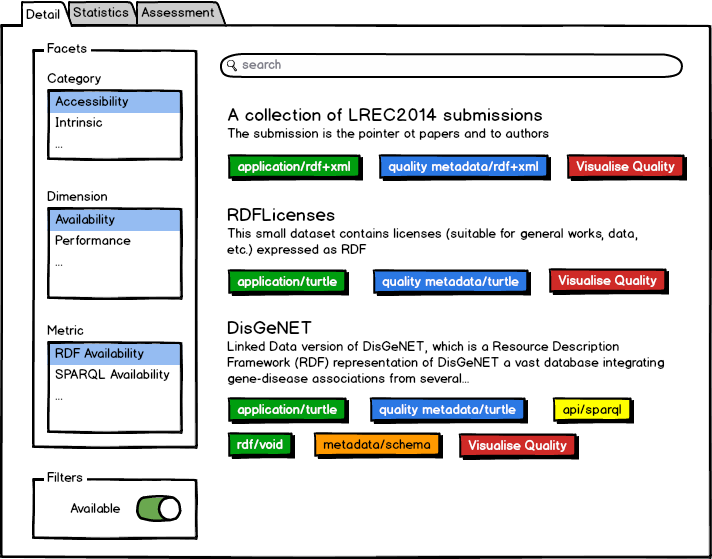
\includegraphics[width=\textwidth]{images/uiDetailsTab.png} 
\caption{Mockup for the Details Tab} 
\label{fig:uiDetailsTab}
\end{figure*}

\subsubsection{Statistics Tab}
The Quality Assessment Framework Web-UI will also give the opportunity to its users to visualise statistical information about a dataset quality.
The Statistical Tab (Figure~\ref{fig:uiStatisticsTab}) will present the user with a number of graphs (cf. Visualisation Layer – \todo{CL@JD: broken ref}Figure~\ref{fig:qualityFramwork} for the description of the different visualisation graphs).
Users can compare different datasets together or even how a dataset changed in its quality over time.

\begin{figure*}[tbph]
\center
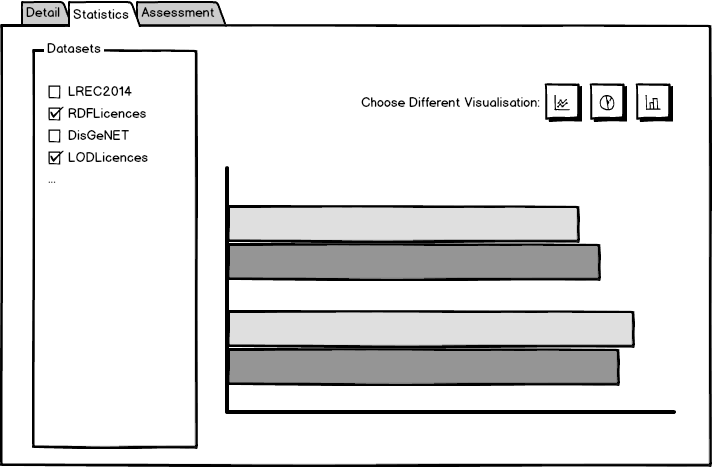
\includegraphics[width=\textwidth]{images/uiStatisticsTab.png} 
\caption{Mockup for the Statistics Tab} 
\label{fig:uiStatisticsTab}
\end{figure*}

\subsubsection{Visualisation Layer}
\label{sec:vislayer_hla}
CubeViz is an extension of the OntoWiki\footnote{\url{http://ontowiki.eu/Welcome}} data wiki for visualising data cubes (observation instances).
Figures~\ref{fig:hor_chart},~\ref{fig:ver_chart},~\ref{fig:rad_chart}, and~\ref{fig:line_chart} depicts four different CubeViz chart visualisations from computed quality metadata\footnote{The quality metadata used can be found in \url{https://raw.githubusercontent.com/diachron/quality/master/src/test/resources/cube_qg.trig}}.  While these are generic chart types, we briefly discuss their specific suitability for data quality analysis.

\begin{figure*}[tbph]
\center
  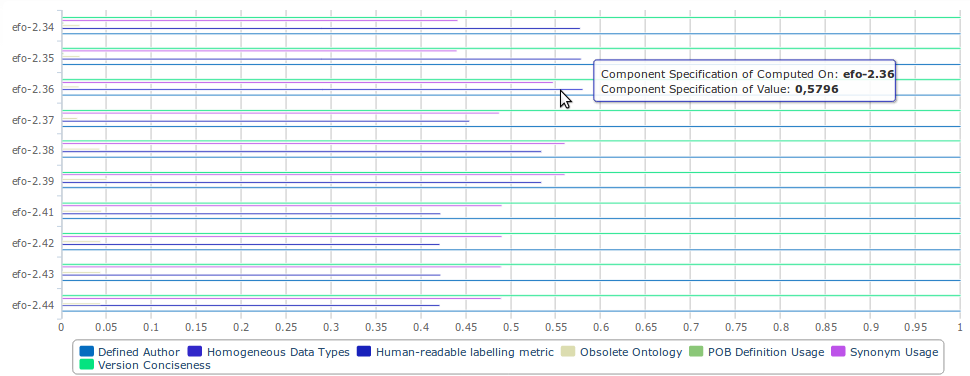
\includegraphics[scale=0.3]{images/cube_1.png}
\caption{Horizontal Bar Chart} 
  \label{fig:hor_chart}
\end{figure*}

\begin{figure*}[tbph]
\center
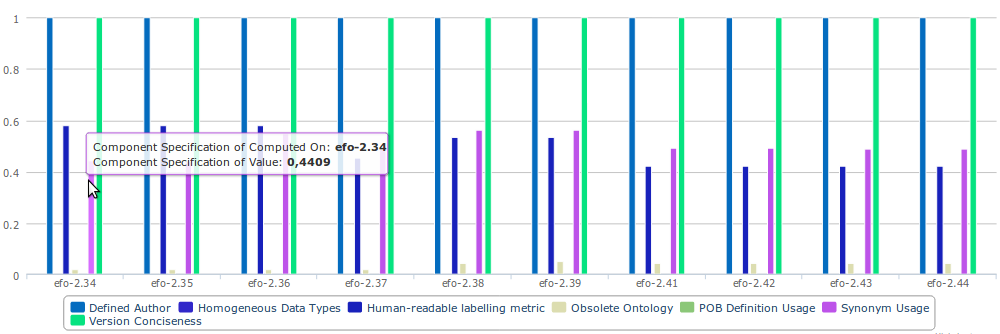
\includegraphics[scale=0.3]{images/cube_2.png} 
\caption{Vertical Bar Chart} 
\label{fig:ver_chart}
\end{figure*}

\begin{figure*}[tbph]
\center
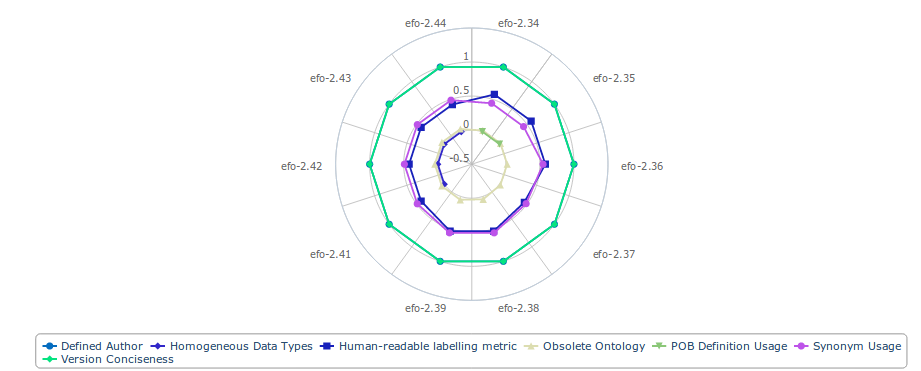
\includegraphics[scale=0.3]{images/cube_3.png} 
\caption{Radar Chart} 
\label{fig:rad_chart}
\end{figure*}

\begin{figure*}[tbph]
\center
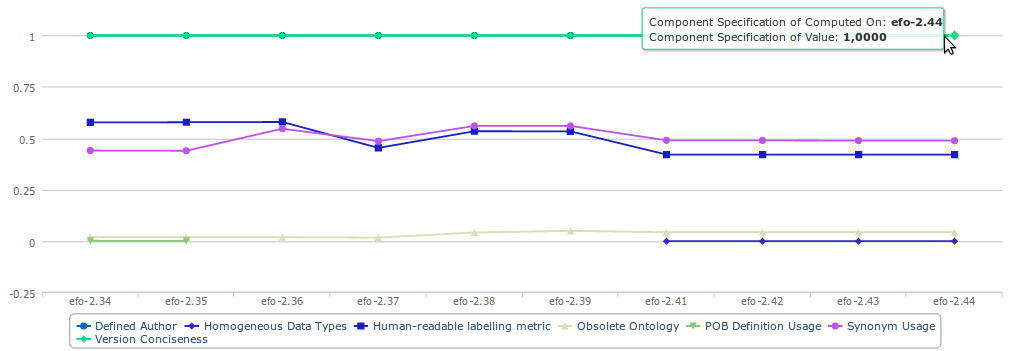
\includegraphics[scale=0.3]{images/cube_4.png} 
\caption{Lines Plot} 
\label{fig:line_chart}
\end{figure*}

A \emph{horizontal bar} represents each metric (Figure~\ref{fig:hor_chart}) and shows its value (x-axis) with respect to the dataset (y-axis).
Here, the different “datasets” analysed are actually successive revisions of one dataset.
This chart provides a clear view of how the value associated to each one of the measured metrics changes as the dataset evolves.
The horizontal layout is appropriate when the range of metric values is wide, and the number of different datasets is relatively small.

Similar to the horizontal bars chart, the \emph{vertical bar chart} (Figure~\ref{fig:ver_chart}) allows the user to compare the values computed for each of the metrics (y-axis), with respect to the dataset (x-axis).
In contrast with its horizontal counterpart, this chart is more appropriate when there are many datasets analysed but the range of metric values is not so wide.

In the \emph{radar chart} (Figure~\ref{fig:rad_chart}), the datasets are represented as slices of a circle and the values corresponding to the metrics are depicted as points and lines of a particular colour.
This chart provides a clear view of how the values of the metric differ from each other for each particular dataset. 
Furthermore, it allows one to assess the overall quality of a dataset, by showing whether the values of the metrics are concentrated around sections of the circle regarded as “good” or “bad”.

The lines plot (Figure~\ref{fig:line_chart}), lists the different datasets against the values of the metrics.
Here, where “different datasets” are actually different revisions in the evolution of one dataset, this plot provides a comparison of the evolution of the quality of the dataset, with respect to each metric.
The lines emphasise the points where the values of the metrics changed noticeably from one version to the next.


\subsubsection{Assessment Tab}
The Quality Framework Web-UI will also allow users to assess datasets for their quality.
Figure~\ref{fig:uiAssessementTab} shows a mockup of how the Assessment Tab will look like.
The user is guided step by step to assess a dataset:
\begin{enumerate}
\item The user chooses the dataset to be assessed or give a dataset URI;
\item User decides what metrics to be assessed;
\item User decides if a quality problem report is required, which would allow the user to semi-automatically clean up the data (cf. Deliverable 3.1);
\item User clicks the \emph{assess} button to start assessing the chosen datasets.
\end{enumerate}

\begin{figure*}[tbph]
\center
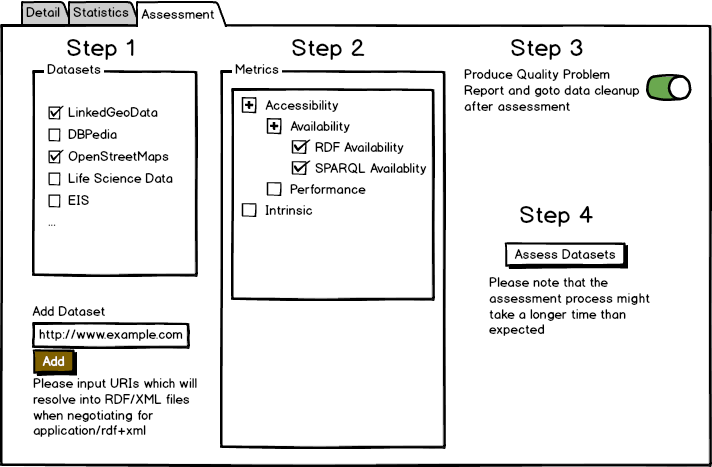
\includegraphics[width=\textwidth]{images/uiAssessmentTab.png} 
\caption{Mockup for the Assessment Tab} 
\label{fig:uiAssessementTab}
\end{figure*}

% describe the proposed UI mockups
%!TEX root = ../../diachron-D5_2.tex

\subsection{Ranking of Quality-Computed Datasets}
\label{sec:Ranking} 
Tools for data consumers, such as CKAN, usually provide features such as faceted browsing and sorting, in order to allow prospective dataset users to search within the large dataset archive.
Using faceted browsing, datasets could be filtered according to tags or values of metadata properties.
The datasets could also be ranked or sorted according to values of properties such as relevance, size or the date of last modification.
With many datasets available, filtering or ranking by quality can become a challenge.
Talking about ``quality'' as a whole might not make sense, as different aspects of quality matter for different applications.
It does, however, make sense to restrict quality-based filtering or ranking to those quality categories and/or dimensions that are relevant in the given situation, or to assign custom weights to different dimensions, and compute the overall quality as a weighted sum.
The daQ vocabulary provides flexible filtering and ranking possibilities in that it facilitates access to dataset quality metrics in these different dimensions and thus facilitates the (re)computation of custom aggregated metrics derived from base metrics.
To keep quality metrics information easily accessible, each assessed dataset contains the relevant daQ metadata graph in the dataset itself.
We provide two ranking possibilities to the user: (i) Unbiased Automatic Quality Ranking, and (ii) User-Driven Quality Ranking.

\subsubsection{Unbiased Automatic Quality Ranking}
We aim to achieve a quality-biased ranking of LOD datasets, promoting:
\begin{enumerate}
\item High quality datasets;
\item Datasets on which a larger number of quality metrics is calculated. 
\end{enumerate}
Therefore, datasets of poor quality but having more quality metadata might end up ranked higher than those with excellent quality on the only metric assessed on.
Publishers might be doubtful about the data they publish and they will hide their doubt in the dataset itself.
One possibility is that the publishers might hide this psychological nature by claiming that their dataset is of good quality in certain aspects.
Quality assessment frameworks should not only be about positive or negative assertions of a dataset, but also it should place the publishers` doubts in the assertion spectrum.
With our proposed ranking algorithm we do not just promote those datasets that have a high value to one particular metric, but we promote those datasets, which although might lack in particular metric assessment, have more coverage of assessed metrics.

The approach we take for ranking takes into consideration the total number of metrics assessed by the most complete dataset available in the datastore\footnote{We are assuming that the metrics used are common to all datasets in the domain}.
It also takes into consideration any facet filters chosen by the user, enabling the dynamic change of weights and thus the final ranking.
Consider $F_{m} = \lbrace m_{1},m_{2},\dots,m_{n} \rbrace$ where $F_{m}$ is the set of all metrics $m$ available.
The ranking algorithm is split into a number of steps:
\begin{enumerate}
\item Get the total number of metrics assessed ($n$);
\item Adjust weight for those metrics selected in the facet (Definition~\ref{def:weight_adjustment});
\item Adjust weight for the rest of the metrics (Definition~\ref{def:weight_adjustment_smaller});
\item Calculate the metric value by weight to find out ranking (Definition~\ref{def:ranking}) and rank;
\end{enumerate}

\subsubsection{Weight Assignment}
The weight assignment is the most crucial aspect of the ranking algorithm.
It should be evenly distributed amongst the chosen (filtered) metrics, whilst also giving a share of the weight to the other metrics.
In this way we ensure the quality-bias ranking and promote not just the high quality datasets, but also giving a smaller share to those that give more information about quality than others.
In Definition~\ref{def:weight_adjustment} we calculate a weight value for the number of metrics chosen ($\#X$) i.e. those metrics given a preference by the user.
Together with the number of metrics chosen, we add 1 to represent a small share which will be divided equally with the rest of the metrics ($\#\overline{X}$ represents the metrics not chosen).
This is defined in Definition~\ref{def:weight_adjustment_smaller}.
To explain this in a simpler manner, if we have five metrics and only one was chosen, then the chosen metric will have a weight of 0.5 whilst the rest will have 0.5 shared equally (i.e. 0.125).

\begin{Def1}
\label{def:weight_adjustment}
\begin{align*}
Let~X~\subseteq~(F_{m}~\cup~\emptyset) \\
\theta = \frac{1}{(\#X + 1)}
\end{align*}
\end{Def1}

\begin{Def1}
\label{def:weight_adjustment_smaller}
\begin{align*}
Let~\overline{X}~=~(X~\cap~{F_{m}}^{\complement}) \\
\rho = \frac{1}{((\#X + 1) \times \#\overline{X})}
\end{align*}
\end{Def1}

\subsubsection{Ranking Datasets}
After the weights have been distributed, the ranking algorithm retrieves all the metric values from the quality graph.
The values of chosen metrics i.e. the set $X$, are added together and multiplied by the weight $\theta$.
Similarly, the complement set ($\overline{X}$) are multiplied by the weight $\rho$.
These two are added together which gives us a value $\tau$ for the dataset (Definition~\ref{def:ranking}).
This is repeated for all possible datasets and then are ranked accordingly.
\begin{Def1}
\label{def:ranking}
\begin{align*}
\tau = (\sum_{i~=~0}^{\#X} X_{i}~.~\theta) + (\sum_{i~=~0}^{\#\overline{X}} \overline{X_{i}}~.~\rho)
\end{align*}
\end{Def1}

Listing~\ref{lst:rank_sparql} shows a typical configuration of the retrieval of metric assessment values from the Quality Graph.
In this query the metric value of the latest observation is taken into consideration.
\lstinputlisting[caption={Retrieving metric assessment value from the Quality Graph.},label=lst:rank_sparql, language=SPARQL]{listings/ret_value.sparql}

\subsubsection{Ranking Example}
In the following subsection we introduce an example to further help the reader to understand how ranking will work.
Consider the following dataset scenario in Table~\ref{tbl:datasets}.
In our datastore we have four datasets each having a Quality Graph with a number of assessed metrics and their values.
\textit{Dataset D} has been assessed by all eight metrics whilst the others have been assessed with six, five and five respectively.
\begin{table}[tbph]
\center
    \begin{tabular}{|l|l|l|l|l|}
    \hline
    \textbf{Metric} & \textbf{Dataset A} & \textbf{Dataset B} & \textbf{Dataset C} & \textbf{Dataset D} \\   \hline
    A      & 0.2       & 0.9       & 0.5       & 0.3       \\  \hline
    B      & 0.5       & 0.9       & 0.8       & 0.4       \\  \hline
    C      & 0.9       & 0.3       & 0.7       & 0.7       \\  \hline
    D      & 0.8       & -         & 0.9       & 0.1       \\  \hline
    E      & 0.7       & -         & 0.4       & 0.1       \\  \hline
    F      & -         & 0.2       & -         & 0.5       \\  \hline
    G      & -         & 0.8       & -         & 0.9       \\  \hline
    H      & 0.3       & -         & -         & 0.9       \\  \hline
    \end{tabular}
    \label{tbl:datasets}
    \caption{Dataset example}
\end{table}

In Table~\ref{tbl:dataset_ranking} we show how the ranking value $\tau$ would dynamically change for different scenarios.
Initially, no filter is chosen by the user.
A possible scenario for this is on page load.
When no filter is chosen (in this example) all weights have a $\rho$ value of 0.125.
\textit{Dataset D} will be ranked first, followed by \textit{Dataset A}, \textit{Dataset C} and \textit{Dataset B}.
This shows that although at first glance it seems that \textit{Dataset B} is a high quality dataset (three out of five assess quality metrics are over 0.8), it got penalised by the fact that other datasets had more quality metadata about their dataset.
The single filters \textbf{A} and \textbf{E} gave expected results, with \textit{Dataset B} and \textit{Dataset A} being top ranked respectively. 
The multiple filter \textbf{A,B} also gave expected results, with \textit{Dataset D} being ranked third ahead of \textit{Dataset A} due to the it having more quality metadata.
More examples of different scenarios are in the Table~\ref{tbl:dataset_ranking}, where the blue coloured cells shows the top-ranked dataset.
\begin{table}[tbph]
    \begin{tabular}{|l|l|l|l|l|l|l|l|}
    \hline
    \textbf{Chosen Filter} & \textbf{Dataset A}                                 & \textbf{Dataset B}                                 & \textbf{Dataset C}  & \textbf{Dataset D}                                  & ~ & $\theta$ & $\rho$ \\  \hline
     \textbf{No Filter}     & 0.425                                     & 0.3875                                    & 0.4125     &      \cellcolor{blue!25} 0.4875 & ~ & 1                   & 0.125             \\  \hline
     \textbf{A}             & 0.32857143                                & \cellcolor{blue!25} 0.60714286 & 0.45       & 0.40714286                                 & ~ & 0.5                 & 0.07142857        \\  \hline
    \textbf{E}             & \cellcolor{blue!25} 0.54285714 & 0.22142857                                & 0.40714286 & 0.32142857                                 & ~ & 0.5                 & 0.07142857        \\  \hline
     \textbf{A,B}           & 0.38333333                                & \cellcolor{blue!25} 0.67222222 & 0.54444444 & 0.41111111                                 & ~ & 0.33333333          & 0.05555556        \\  \hline
    \textbf{A,B,C}         & 0.49                                      & \cellcolor{blue!25} 0.575      & 0.565      & 0.475                                      & ~ & 0.25                & 0.05              \\  \hline
    \textbf{A,E}           & \cellcolor{blue!25} 0.43888889 & 0.42222222                                & 0.43333333 & 0.32777778                                 & ~ & 0.33333333          & 0.05555556        \\  \hline
    \textbf{B,D,E,H}       & \cellcolor{blue!25} 0.515      & 0.29                                      & 0.48       & 0.42                                       & ~ & 0.2                 & 0.05              \\  \hline
    \end{tabular}
    \label{tbl:dataset_ranking}
    \caption{Dataset Ranking for different Scenarios}
\end{table}

\subsubsection{User-Driven Quality Ranking}
We will also allow the user to define custom weights to their preferred metrics.
At the moment we are also investigating how ranking can be applied to the category and dimension levels.
%!TEX root = ../../diachron-D5_2.tex

\section{Crawling Service}
\label{sec:CrawlingService} 

%!TEX root = ../../diachron-D5_2.tex

\section{Conclusions}
\label{sec:Conclusion} 

This document describes the software prototype for crawling, ranking and appraisal services which is required as part of the DoW in M16 of the project.
It provides a detailed high level description on the Quality Assessment Framework (Section~\ref{sec:HLA}), which provides the basis of this prototype.

During the initial phase, pilot partners identified the required metrics for their use cases (cf. Deliverable 5.1~\cite{diachron-d5.1}).
Having these in mind, a framework was identified to facilitate the quality assessment of the pilots' datasets together with providing enough metadata to enable the crawling and ranking of these datasets.
After describing the Quality Assessment framework, Assessment and Ranking services were described in Section~\ref{sec:Ranking} whilst Crawling services were described in Section~\ref{sec:CrawlingService}.
\todo{CL: Can't say ``runnable'' unless you put a downloadable executable file there}The sources of the prototype of the assessment framework can be found at \url{https://github.com/diachron/quality}\footnote{Please note that this URL can change without any notice.}.

The approach taken in the QA framework is a generic pluggable approach, therefore it can be used even beyond the scope of DIACHRON.
Additionally, a number of research tasks were also addressed in the framework, particularly the representation of quality metadata.

\printbibliography

%%%%%%%%%%%%%%%%%%%%%%%%%%%%%%%%%%%%%%%%%%%%%%%%%
% ...and in the words of Terry Tibbs:
% Thank you, goodnight -- much love.
%%%%%%%%%%%%%%%%%%%%%%%%%%%%%%%%%%%%%%%%%%%%%%%%%

\end{document}

%%% Local Variables: 
%%% mode: latex
%%% TeX-master: t
%%% LaTeX-biblatex-use-Biber: nil
%%% End: 
